\documentclass[oneside, 12pt, french]{book}
% !TEX encoding = UTF-8 Unicode
% LaTeX Preamble
% Author : Gabriel Crépeault-Cauchon
% Last update : 08/09/2019
% ---------------------------------------------
% BEGINNING OF PREAMBLE
% ---------------------------------------------
% Encoding packages
\usepackage[utf8]{inputenc}
\usepackage[T1]{fontenc}
\usepackage{babel}
\usepackage{lmodern}

% HYPERREF (URL's and Link options)
\usepackage{hyperref}
\hypersetup{colorlinks = true, urlcolor = red!60!black, linkcolor = red!60!black}

% POLICY (choose one of them)
%	\usepackage{concrete}
%	\usepackage{mathpazo}
%	\usepackage{frcursive} %% permet d'écrire en lettres attachées
 \usepackage{aeguill}
% 	\usepackage{mathptmx}
%	\usepackage{fourier} 

% Mathematics configuration
\usepackage{amsmath,amsthm,amssymb,latexsym,amsfonts}
\usepackage{empheq}
\usepackage{numprint}
\usepackage{dsfont} 


% Tcolorbox config
\usepackage{tcolorbox}
\tcbuselibrary{xparse}
\tcbuselibrary{breakable}

% Définition Boite pour exemple
\newcounter{ex}[section]
\DeclareTColorBox{exemple}{ o }% #1 parameter
{colframe=green!20!black,colback=green!5!white, % color of the box
breakable, pad at break*=0mm, % to split the box
before title = {\textbf{Exemple \stepcounter{ex} \arabic{chapter}.\arabic{section}.\arabic{ex} }},
IfValueTF = {#1}{title= {#1}}{title= \hphantom},
after title = {\large \hfill \faWrench}
}

%% Définition boite pour définition
\newcounter{def}[section]
\DeclareTColorBox{definition}{ o }% #1 parameter
{colframe=blue!60!green,colback=blue!5!white, % color of the box
breakable, pad at break*=0mm, % to split the box
before title = {\textbf{Définition \stepcounter{def} \arabic{chapter}.\arabic{section}.\arabic{def} }},
title = {#1},
after title = {\large \hfill \faBook}
}

\DeclareTColorBox{note}{ o }
    {colframe=black,
     colback=white,
     sharp corners,
     pad at break*=0mm,
     IfValueTF={#1}{title={#1}, fonttitle=\bfseries}{title=Note, fonttitle=\bfseries}}


% Graphics and picture import Packages
\usepackage{graphicx}
\usepackage{pict2e}

% insert PDF package
\usepackage{pdfpages}

% Color package
\usepackage{color, soulutf8, colortbl}

% Mathematics table
\usepackage{array}   % for \newcolumntype macro
\newcolumntype{L}{>{$}l<{$}} % math-mode version of "l" column type

% usefull shortcut for colored text
\newcommand{\orange}{\textcolor{orange}}
\newcommand{\red}{\textcolor{red}}
\newcommand{\cyan}{\textcolor{cyan}}
\newcommand{\blue}{\textcolor{blue}}
\newcommand{\green}{\textcolor{green}}
\newcommand{\darkgreen}{\textcolor{darkgreen}}
\newcommand{\purple}{\textcolor{magenta}}
\newcommand{\yellow}{\textcolor{yellow}}

% Colors define
\definecolor{darkgreen}{RGB}{37, 128, 40}
\definecolor{tocColor}{HTML}{8A2507}

% Custum enumerate & itemize Package
\usepackage{enumitem}
% French Setup for itemize function
\frenchbsetup{StandardItemLabels=true}

% Mathematics shortcut
\usepackage{cancel}
\newcommand{\reels}{\mathbb{R}}
\newcommand{\entiers}{\mathbb{Z}}
\newcommand{\naturels}{\mathbb{N}}
\newcommand{\eval}{\biggr \rvert}
\newcommand{\esp}[1]{\mathrm{E} \left[ #1 \right]} % espérance
\newcommand{\variance}[1]{\mathrm{Var} \left( #1 \right)} % variance
\newcommand{\covar}[1]{\mathrm{Cov} \left( #1 \right)} % variance
\newcommand{\prob}[1]{\Pr \left( #1 \right)} % probabilité entre parenthèses
\newcommand{\laplace}{\mathcal{L}}
\newcommand{\matr}[1]{\mathbf{#1}} % Notation matricielle
\DeclareMathOperator{\Tr}{Tr}
\newcommand{\fgp}{\mathcal{P}}
\DeclareMathOperator{\Adj}{Adj}
\newcommand{\derivee}[1]{\frac{\partial}{\partial #1}}
\newcommand{\indic}[1]{\mathds{1}_{\{ #1 \}}}
\newcommand{\VaR}[2][k]{\mathrm{VaR}_{#1}{\left( #2 \right)}}
\newcommand{\TVaR}[2][k]{\mathrm{TVaR}_{#1}{\left( #2 \right)}}


% Matricial anotation for math symbols (\bm{•})
% à enlever éventuellement, j'ai ajouté la macro \matr{} à la place.
\usepackage{bm}

% Actuarial notation package
\usepackage{actuarialsymbol}
\usepackage{actuarialangle}

% To indicate equation number on a specific line in align environment
\newcommand\numberthis{\addtocounter{equation}{1}\tag{\theequation}}

% Other shortcut
\newcommand{\p}{\paragraph{}}
\newcommand{\n}{\newline}

% source : https://tex.stackexchange.com/questions/112576/math-mode-in-tabular-without-having-to-use-everywhere



% Special symbols package
 \usepackage[tikz]{bclogo}
\usepackage{fontawesome}

% Retire l'indentation automatique de Latex
\setlength{\parindent}{0pt}

% Utilisé pour la page couverture
\usepackage[absolute]{textpos} % Textblock environement
\usepackage{anyfontsize} % Avoir un gros titre
\usepackage{titling} % Avoir un gros titre
\usepackage{changepage} % ajustwidth environement

% Pour afficher du code
\usepackage{listings}

\definecolor{codegray}{gray}{0.9}
\newcommand{\code}[1]{\colorbox{codegray}{\texttt{#1}}}

\definecolor{insideBlackTerminal}{RGB}{33,33,33}
% Set Language
% \lstset{
%     language={bash},
%     basicstyle=\small\ttfamily\color{white}, % Global Code Style
%     captionpos=b, % Position of the Caption (t for top, b for bottom)
%     extendedchars=true, % Allows 256 instead of 128 ASCII characters
%     tabsize=2, % number of spaces indented when discovering a tab 
%     columns=fixed, % make all characters equal width
%     keepspaces=true, % does not ignore spaces to fit width, convert tabs to spaces
%     showstringspaces=false, % lets spaces in strings appear as real spaces
%     breaklines=true, % wrap lines if they don't fit
%     frame=single, % draw a frame at the top, right, left and bottom of the listing
%     numberstyle=\tiny\ttfamily, % style of the line numbers
%     % commentstyle=\color{red}, % style of comments
%     % keywordstyle=\color{red}, % style of keywords
%     % stringstyle=\color{red}, % style of strings
%     backgroundcolor = \color{insideBlackTerminal},
%     rulecolor=\color{red}
% }

\usepackage{lstlinebgrd}
\definecolor{grayComment}{HTML}{8D90B8}
\lstset{
language=R,                     % the language of the code
basicstyle=\ttfamily, % the size of the fonts that are used for the code
% numbers=left,                   % where to put the line-numbers
% numberstyle=\color{blue},  % the style that is used for the line-numbers
% stepnumber=1,                   % the step between two line-numbers. If it is 1, each line
% will be numbered
numbersep=5pt,                  % how far the line-numbers are from the code
backgroundcolor=\color{white},  % choose the background color. You must add \usepackage{color}
linebackgroundcolor=\color{white},
showspaces=false,               % show spaces adding particular underscores
showstringspaces=false,         % underline spaces within strings
showtabs=false,                 % show tabs within strings adding particular underscores
frame=single,                   % adds a frame around the code
rulecolor=\color{black},        % if not set, the frame-color may be changed on line-breaks within not-black text (e.g. commens (green here))
tabsize=2,                      % sets default tabsize to 2 spaces
captionpos=b,                   % sets the caption-position to bottom
breaklines=true,                % sets automatic line breaking
breakatwhitespace=false,        % sets if automatic breaks should only happen at whitespace
%   keywordstyle=\color{functionR},      % keyword style
commentstyle=\color[HTML]{9F0808},  %\color[HTML]{8D90B8},   % comment style
%   stringstyle=\color[HTML]{1D9507},      % string literal style
moredelim=**[is][\color{grayComment}]{@}{@}, % couleur manuel
literate=%
{à}{{\`a}}1
{é}{{\'e}}1
{è}{{\`e}}1
} 




















































% ---------------------------------------------
% END OF PREAMBLE
% ---------------------------------------------

\newcommand{\TITLE}{%
Guide de survie  %The blank line after is needed.

\vspace{3mm}
en Actuariat
}
\newcommand{\AUTHORS}{%
Gabriel Crépeault-Cauchon \href{https://github.com/gabrielcrepeault}{\faGithub}  \href{https://www.linkedin.com/in/gabrielcrepeault/}{\faLinkedinSquare}  \\
Nicholas Langevin  \href{https://github.com/NicholasLangevin}{\faGithub}  \href{https://www.linkedin.com/in/nicholas-langevin-216474182/}{\faLinkedinSquare} \\
}

\begin{document}
% Page titre et table des matières
% Page couverture du document de reference

\pagestyle{empty}

\textblockorigin{0mm}{0mm}
\setlength{\parindent}{0mm}

\begin{textblock*}{\paperwidth}(0mm,0mm)
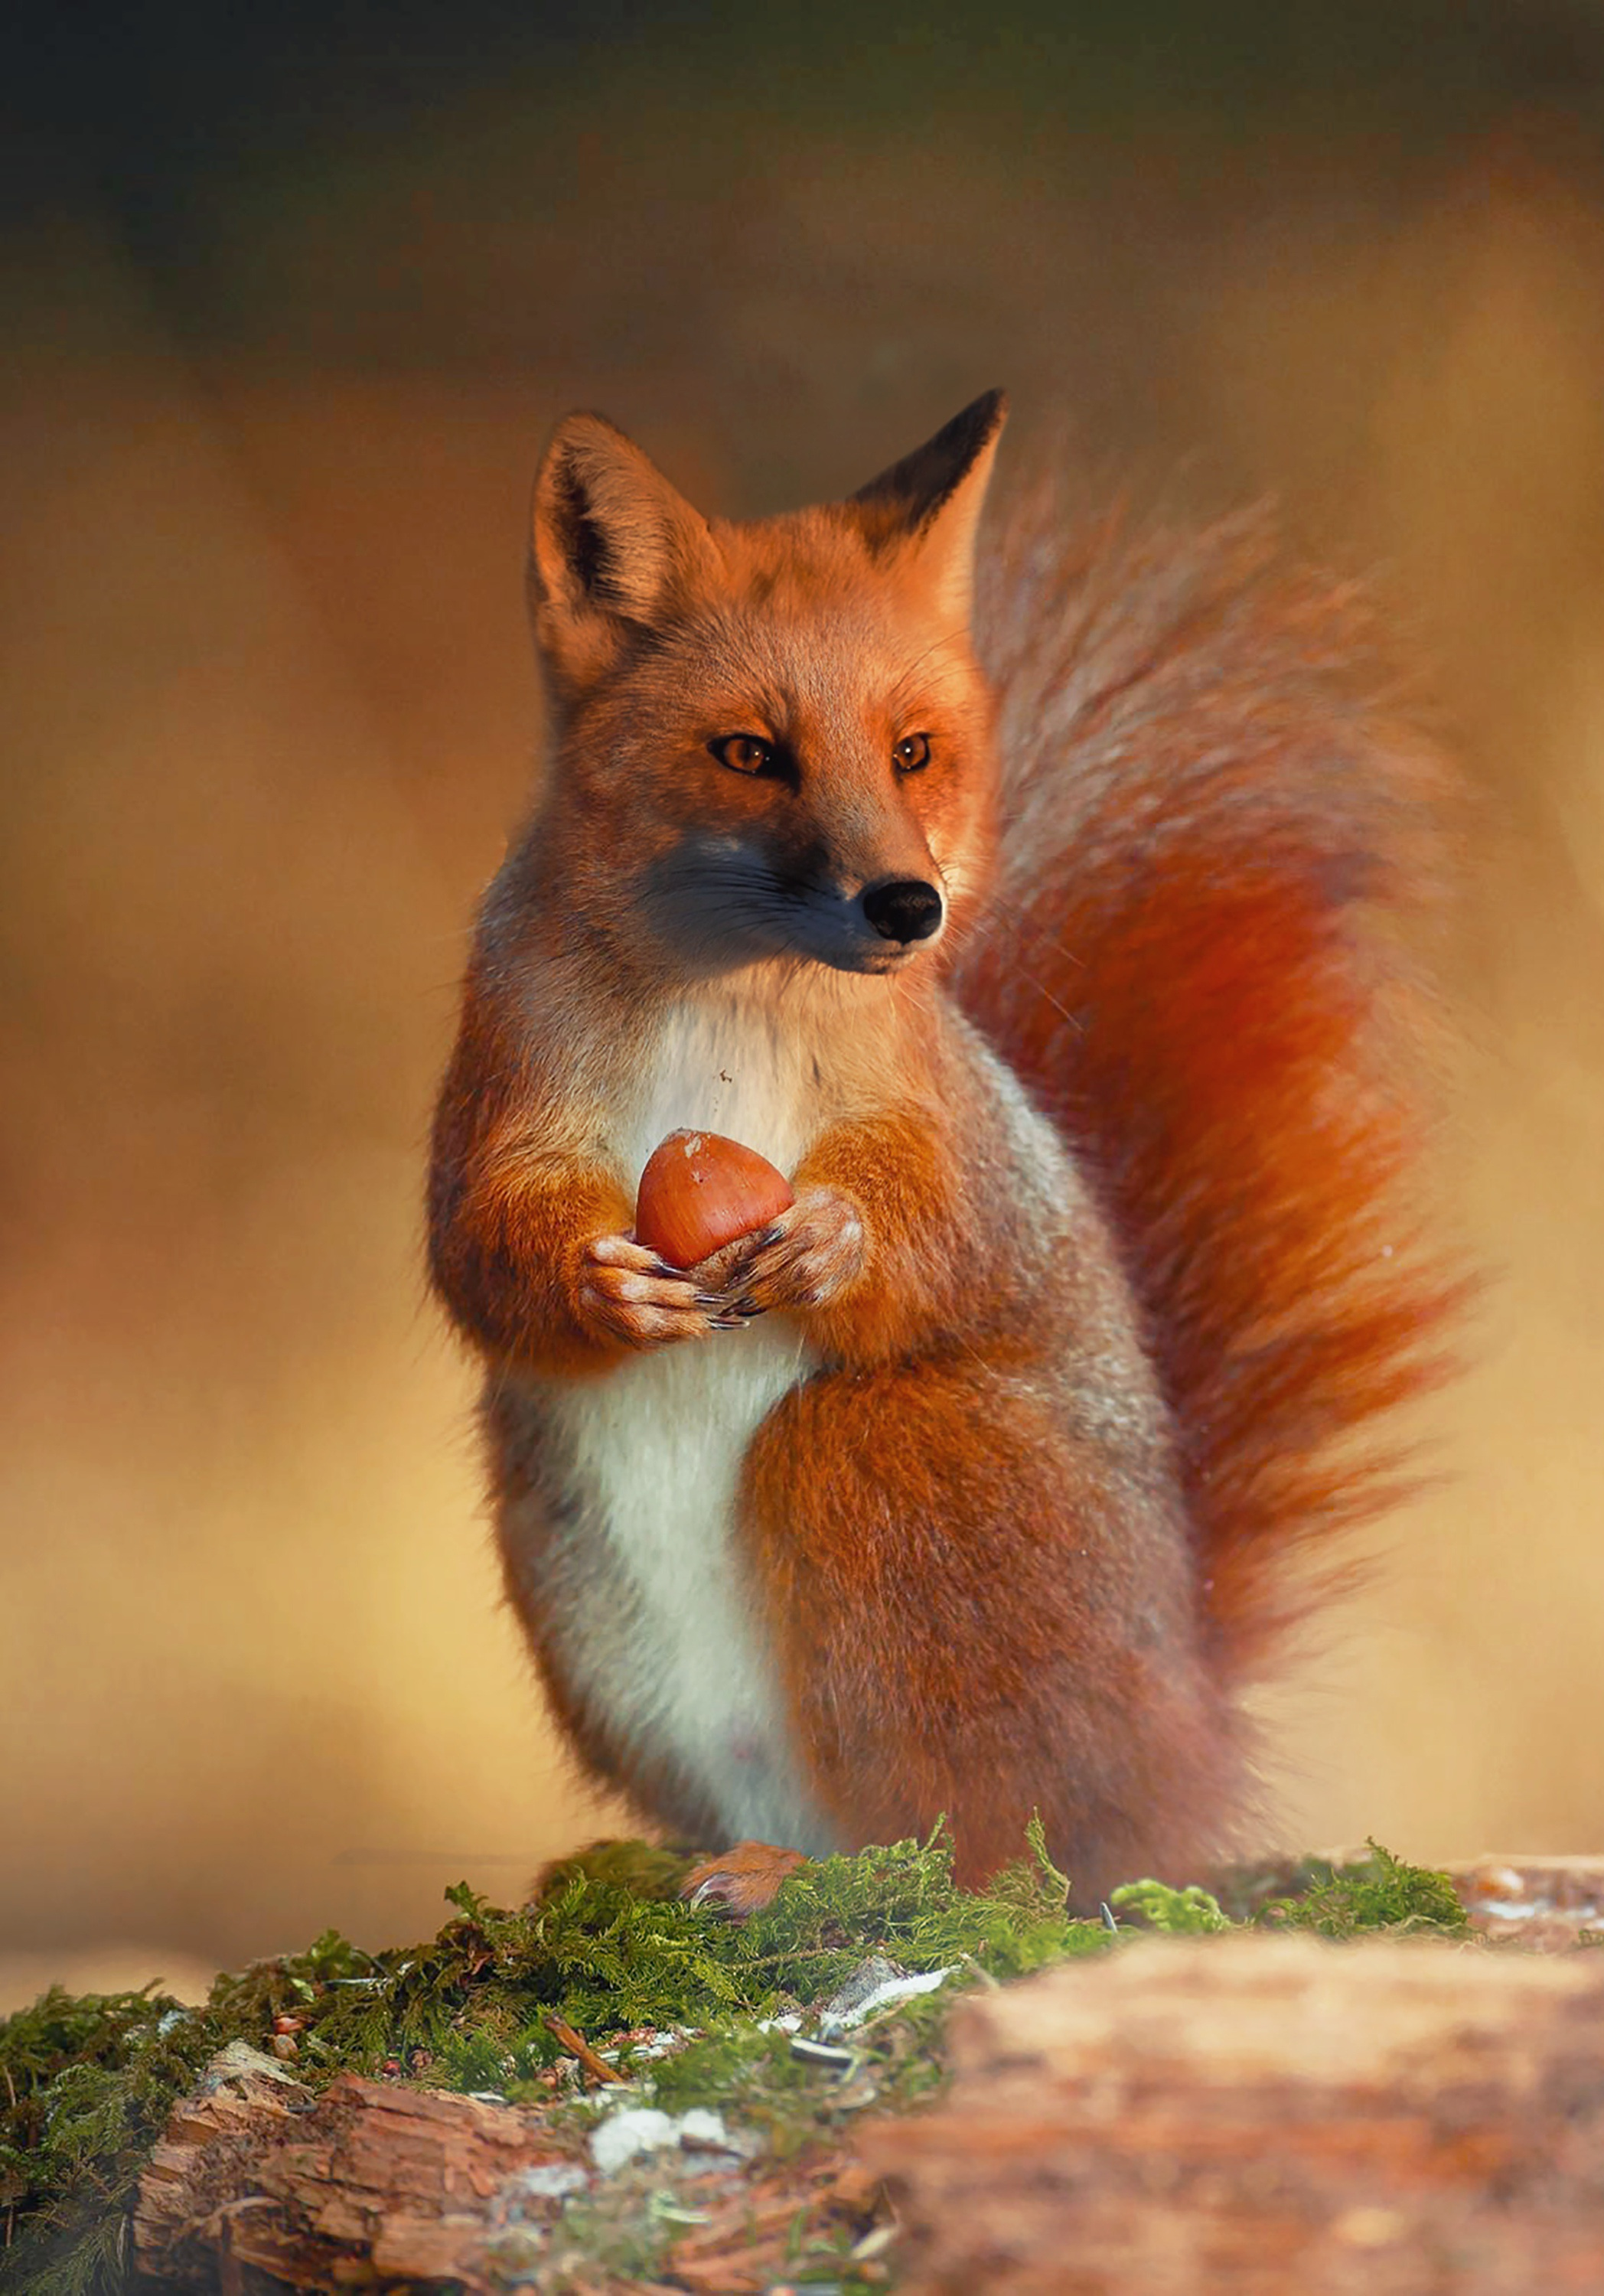
\includegraphics[height=11in, width=\paperwidth]{src/GuideEnActuariat/couverture.jpg} \\
\end{textblock*}

\begin{textblock*}{500mm}(30mm,10mm)
\sffamily
\bfseries\fontsize{52}{42}\selectfont
{ \color{white} 
\TITLE
}
\end{textblock*}

\null\newpage

% ------------------------------------------
% Deuxième page : présentation des auteurs et liens vers le dépôt Github du guide
% ------------------------------------------
\begin{textblock*}{\paperwidth}(20mm,40mm)
\raggedright
\sffamily
\bfseries\fontsize{52}{42}\selectfont
\TITLE
\end{textblock*}

\begin{textblock*}{\paperwidth}(20mm,100mm)
\bfseries\fontsize{15}{15}\selectfont
\raggedright
\AUTHORS
\end{textblock*}


\begin{textblock*}{\paperwidth}(20mm,210mm)
\raggedright
\sffamily
\bfseries\fontsize{10}{10}\selectfont
\href{https://github.com/NicholasLangevin/Guide_de_survie_en_actuariat}{Dépôt officiel de ce document} \\
Dernière mise à jour : \today
\end{textblock*}

\null\newpage


\frontmatter % PRÉFACE
\chapter{Introduction}

On explique ici les motivations du document
\chapter{Liste des collaborateurs}
Voici la liste des personnes ayant collaboré à ce document : 
\begin{itemize}
\item Gabriel Crépeault-Cauchon
\item Nicholas Langeevin
\end{itemize}

{
    \hypersetup{linkcolor=tocColor}
    \bfseries % Pas encore sur si c'est plus beau...
    \tableofcontents
}
\newpage
% ------

\mainmatter % début du document principal

% FONDEMENTS MATHÉMATIQUES
\part{Fondements mathématiques utiles}

\chapter{Notions de calcul différentiel et calcul intégral}

\section{Règles de dérivation}
Dans le tableau, on utilise $k \in \reels$ ou $n$ pour parler d'une constante, $u$, $v$ ou $w$ pour parler d'une fonction.

\begin{tabular}{|L | L |}
% Voir préambule, L est un type de colonne défini (custom) qui place le texte entre $•$
\hline
\text{Fonction}	& \text{Dérivée} \\\hline \hline
f(x) = k	& f'(x) = 0 \\\hline
f(x) = k x	& f'(x) = k \\\hline
f(x) = x^{n}	& f'(x) = n x^{n-1} \\\hline
f(x) = k g(x)	& f'(x) = k g'(x) \\\hline
f(x) = g(x) \pm h(x)	& f'(x) = g'(x) \pm h'(x) \\\hline
f(x) = g(x) \cdot h(x)	& f'(x) = g'(x) \cdot h(x) + g(x) \cdot h'(x) \\\hline
f(x) = \frac{g(x)}{h(x)}	& f'(x) = \frac{g'(x) h(x) - g(x) h'(x)}{h(x)^2} \\\hline
f(x) = g(x)^{n}	& f'(x) = n \cdot g(x)^{n-1} \cdot g'(x) \\\hline
f(x) = k^{g(x)}	& f'(x) = k^{g(x)} \ln k \cdot g'(x) \\\hline
f(x) = e^{g(x)}	& f'(x) = e^{g(x)} \cdot g'(x) \\\hline
f(x) = \ln (g(x)) 	& f'(x) = \frac{g'(x)}{g(x)} \\\hline
\end{tabular}

\label{Chapter:NotionCalculs}

% Chapitre sur l'algèbre linéaire
% Concepts préalables pour le cours STT-2200
\chapter{Algèbre linéaire}

\section{Définition d'un vecteur et une matrice}
\paragraph{Vecteur ligne} Un vecteur ligne $\bm{x}$est un vecteur de dimension $p \times 1$, tel que
\begin{align*}
\matr{x} = 
\begin{bmatrix}
x_1 \\
x_2 \\
... \\
x_p \\
\end{bmatrix}
\end{align*}

\paragraph{Matrice} Une matrice $\matr{A}=[a_{ij}]_{m \times n}$  de dimension $m$ lignes par $n$ colonnes , définie telle que
\begin{equation}
\label{eq:matrice-base}
\matr{A} = 
\begin{bmatrix}
a_{11}    & a_{12}    &  ...   &  a_{1n} \\
a_{21}    & a_{22}    &  ...   &  a_{2n} \\
...    & ...    &  \ddots   &  ... \\
a_{m1}    & a_{m2}    &  ...   &  a_{mn} \\
\end{bmatrix}
\end{equation}


\paragraph{Matrice carrée} Une matrice carrée $\matr{A}$ de dimensions $m \times m$ a autant de lignes que de colonnes.

\paragraph{non-négative} $\matr{A}$ est définie comme \textit{non-négative} si $\matr{x^{\top} A x }\geq 0$, $\forall \matr{x}\in \reels^n$.

\paragraph{positive} $\matr{A}$ est définie comme \textit{positive} si $\matr{x^{\top} A x} > 0$, $\forall \matr{x} \neq 0$.

\paragraph{semi-positive} $\matr{A}$ est définie comme non-négative, mais elle n'est \underline{pas} définie positive.

\paragraph{Orthogonale} $\matr{A}$ est \textit{orthogonale} si elle est non-singulière et $\matr{A}^{-1} = \matr{A}^{\top}$ (voir \autoref{ssec:matrice-inverse} pour définition de $\matr{A}^{-1}$)


\paragraph{Matrice symétrique} La matrice $\matr{A}$ est symétrique si  $a_{ij} = a_{ji}  \ \forall i,j$, i.e
\begin{align*}
\matr{A} = 
\begin{bmatrix}
1     & 2    &  3   \\
2     & 1   & 4 \\
3   & 4   & 1 \\
\end{bmatrix}
\end{align*}

\paragraph{Matrice triangulaire (inférieure ou supérieure)} Une matrice inférieure $\matr{L}$ est constituée de 0 en dessous de la diagonale : 
\begin{align*}
\matr{L} = 
\begin{bmatrix}
1     & 2    &  3   \\
\red{0}     & 1   & 4 \\
\red{0}   & \red{0}   & 1 \\
\end{bmatrix}
\end{align*}

À l'inverse, on peut aussi avoir une matrice triangulaire supérieure $\matr{U}$ , où les éléments en haut de la diagonale sont tous égaux à 0 : 
\begin{align*}
\matr{U} = 
\begin{bmatrix}
1     & \red{0}    &  \red{0}   \\
8     & 3   & \red{0} \\
2   & 3   & 9 \\
\end{bmatrix}
\end{align*}

\paragraph{Matrice diagonale} Une matrice diagonale $\matr{D}$ a des éléments $d_{ii} > 0$ sur sa diagonale seulement. Cette matrice est à la fois triangulaire inférieure et supérieure. i.e.
\begin{align*}
D = 
\begin{bmatrix}
1     & \red{0}    &  \red{0}   \\
\red{0}     & 3   & \red{0} \\
\red{0}   & \red{0}   & 2 \\
\end{bmatrix}
\end{align*}
Un cas spécial de la matrice diagonale est la matrice identité $\matr{I}$, où $\matr{I}_{ii} = 1 ,\ \forall i$, i.e
\begin{equation}
\label{eq:matrice-identite}
\matr{I} = 
\begin{bmatrix}
1     & 0    &  0   \\
0     & 1   & 0 \\
0   & 0   & 1 \\
\end{bmatrix}
\end{equation}


\paragraph{Matrice diagonalisable} Une matrice $\matr{A}_{n\times n}$ est dite \textit{diagonalisable} s'il existe une matrice carrée $\matr{Q}_{n \times n}$ inversible (ou non-singulière) et une matrice $\matr{D}$ diagonale telle que
\begin{equation}
\label{eq:matrice-diagonalisable}
\matr{Q^{-1} A Q = D} \leftrightarrow \matr{A = Q D Q^{-1}}
\end{equation}
(Théorème sur les matrices symétriques) : Toute matrice carrée symétrique est diagonalisable apr uen matrice orthogonale $\matr{Q}$.

\section{Matrice transposée} Soit la matrice $\matr{A}$ définie en \eqref{eq:matrice-base}. On peut trouver la matrice transposée $\matr{A^{\top}}$, où $[a_{ij}] = [a_{ji]}$. \textbf{En d'autres mots, les lignes deviennent des colonnes.}

Voici quelques propriétés intéressantes avec les matrices transposées : 
\begin{itemize}
  \item $\matr{(A^\top)^\top = A}$
  \item $\matr{(A+B)^\top = A^\top + B^\top}$
  \item $\matr{(kA)^\top = kA^\top}$
  \item $\matr{(AB)^\top = B^\top A^\top}$
  \item $\matr{A^\top A}$ et $\matr{A A^\top}$ sont symétriques.
\end{itemize}

\section{Opérations matricielles} Voici une liste non-exhaustive des opérations matricielles possibles. Côté notation, $A$ et $B$ représente des matrices, $c$ re présente une constante
\begin{itemize}
\item $\matr{A + B}  = [a_{ij} + b_{ij}]$
\item $\matr{A - B}  = [a_{ij} - b_{ij}]$
\item $c\matr{A}   = [ca_{ij}]$
\item Produit matriciel :
\begin{equation}
\label{eq:produit-matriciel}
\matr{AB}   = \left[ \sum_{k=1}^p a_{ik} b_{kj}  \right]_{i \times j}
\end{equation}
avec $\matr{A}=[a_{ip}]$ et $B = [b_{pj}]$
\item $\matr{A(B +C) = AB + AC}$
\item $\matr{A^{-1} A = I =A A^{-1}}$, où $I$ est la matrice identité (voir \autoref{eq:matrice-identite}) et $A^{-1}$ est la matrice inverse de $A$ (voir \autoref{ssec:matrice-inverse} au besoin)
\item $(AB)^{-1} = B^{-1} A^{-1}$
\end{itemize}






\section{Trace, déterminant et matrice inverse}
\subsection{Trace d'une matrice}
\label{ssec:trace-matrice}
Soit la matrice carrée $\matr{A}$. On peut trouver la trace de cette matrice en sommant les éléments de sa diagonale, i.e.

\begin{equation}
\label{eq:trace-mat}
\Tr(\matr{A}) = \sum_{i=1}^n a_{ii}
\end{equation} 
\paragraph{Propriétés de la trace d'une matrice}
\begin{itemize}
\item $\Tr(\matr{A+B}) = \Tr(\matr{A}) + \Tr(\matr{B})$
\item $\Tr(\matr{AB}) = \Tr(\matr{BA})$ et $\Tr(\matr{ABC}) = \Tr(\matr{CAB}) = \Tr(\matr{BCA})$
\end{itemize}

\subsection{Déterminant d'une matrice}
\label{ssec:det-matrice}
Soit la matrice carrée $\matr{A}$. On peut trouver le déterminant de $\matr{A}$, noté $\det(\matr{A})$ ou $|\matr{A}|$, avec
\begin{equation}
\det(\matr{A}) =
\begin{vmatrix}
a & b \\
c & d \\
\end{vmatrix} = ad - bc
\end{equation}
De façon générale, lorsque les dimensions de la matrice carrée sont supérieures à 2, on a
\begin{equation}
\label{eq:det-matrice}
\det(A) = \sum_{j=1}^n a_{ij} C_{ij}
\end{equation}
avec $1 \le i \le n$ où $C_{ij}  = (-1)^{i+j} M_{ij}$ et $M_{ij}$ est le déterminant de la nouvelle matrice en enlevant la ligne $i$ et la colonne $j$.

Si la matrice $\matr{A}$ est inversible (ou non-singulière, voir la \autoref{ssec:matrice-inverse}), alors le déterminant aura les propriétés suivantes : 
\begin{itemize}
\item $\det(A^\top)  = \det(A)$
\item $\det(kA)   = k^n \det(A)$
\item $\det(A + B)  \neq \det(A) + \det(B)$
\item $\det(AB)   = \det(A) \det(B)$
\item $\det(A^{-1})  = \frac{1}{\det(AB)} = \det(A)^{-1}$
\end{itemize}

\subsection{Matrice inverse}
\label{ssec:matrice-inverse}
Soit la matrice carrée $\matr{A}$. On peut trouver la matrice inverse $\matr{A}^{-1}$ telle que

\begin{equation}
\label{eq:mat-inverse}
\matr{A}^{-1} = \frac{1}{\det(\matr{A})} \Adj(\matr{A})
\end{equation}
où $\Adj(\matr{A})   = [C_{ij}]_{m \times n}^T$ et  $C_{ij}   = (-1)^{i+j} M_{ij}$.


\section{Décomposition LDU de Choleski}
Soit $\matr{A}$ une matrice carrée symétrique définie positive. Alors, il existe une décomposition unique telle que
\begin{equation}
\label{eq:decomp-choleski}
\matr{A} = \matr{LDU}
\end{equation}
où $\matr{L, D, U}$ sont respectivement des matrices triangulaire inférieure, triangulaire supérieure et diagonale.

\hl{Cette décomposition peut être fortement utile en programmation lorsqu'on fait des opérations sur des matrices, afin de limiter le nombre d'opérations.}

\section{Vecteurs et valeurs propres}
\subsection{Définition}
Soit $\matr{A}$ une matrice carrée. On dit que $\lambda$ est une \textit{valeur propre} de $\matr{A}$ s'il existe un vecteur $\matr{x} \neq 0$ tel que
\begin{equation}
\label{eq:vecteur-propre}
\matr{Ax = \lambda x}
\end{equation}
On appelle le vecteur $\matr{x}$ un \textit{vecteur propre} correspondant à la valeur propre $\lambda$. De plus, l'ensemble des nombres réels $\lambda$ satisfaisant l'\autoref{eq:vecteur-propre} est appelé \textit{spectre} de la matrice $\matr{A}$.

\subsection{Propriétés intéressantes}
Les vecteurs propres et valeurs propres permettent d'avoir plusieurs propriétés appréciables, notamment : 
\begin{itemize}
\item Si $\matr{x}$ est un vecteur propre de $\matr{A}$ correspondant à la valeur propre $\lambda$, alors $c\matr{x}$ sera également un vecteur propre de $\matr{A}$ correspondant à $\lambda$.
\item Si $\matr{A}$ est symétrique et $\matr{x_1}$ et $\matr{x_2}$ sont des vecteurs propres correspondant à des valeurs propres différentes de $\matr{A}$, alors $\matr{x_1}$ et $\matr{x_2}$ sont des vecteurs ortogonaux, i.e. $\matr{x_{1}^{\top} x_2}  =0$.
\item Si $\matr{A}$ a les valeurs propres (pas nécessairement distinctes) $\lambda_1, \dots, \lambda_n$, alors $\det(\matr{A}) = \prod_{i=1}^{n} \lambda_i$ et $\Tr(\matr{A}) = \sum_{i=1}^{n} \lambda_i$.
\end{itemize}

\subsection{Décomposition spectrale} Soit $\matr{A}_{n\times n}$ une matrice symétrique avec les $n$ valeurs propres $\lambda_1, \dots, \lambda_n$. Il existe une matrice orthogonale $\matr{Q}$ telle que
\begin{equation}
\label{eq:decomposition-spectrale}
\matr{A = Q \Lambda Q^{\top}}
\end{equation}
avec $\matr{\Lambda} = diag(\lambda_1, \dots , \lambda_n)$. Cette décomposition est fort utile lorsqu'on veut faire des produits matriciels successifs de la même matrice (appliqué directement dans les chaînes de Markov, voir \autoref{sec:chaine-markov}) : 
\begin{align*}
\matr{AA} & \matr{= Q \Lambda \underbrace{Q^{\top} Q}_{=I} \Lambda Q^{\top} } \\
 & = \matr{Q \Lambda^2 Q^{\top}}
\end{align*}

\section{Dérivées de matrice ou vecteurs}
Voici quelques entités pratiques : 
\begin{align*}
\derivee{\matr{v}} \matr{w^{\top} v} = w
\end{align*}
\begin{align*}
\derivee{\matr{v}} = \matr{v^{\top} A v = (A + A^{\top})v}
\end{align*}
\label{Chapter:AlgebreLineaire}


% UNIVERSITÉ
\part{Matière vue dans le baccalauréat en actuariat}

% Chapitre sur les concepts de probabilité (ACT-1002) et statistiques (ACT-2000)
\chapter{Probabilités et statistiques}

\section{Concepts de probabilité de base}

\subsection{Probabilité conditionnelle}
\paragraph{Définition de base}
\begin{equation}
\label{eq:prob-cond}
\prob{A|B} = \frac{\prob{A \cap B}}{\prob{B}}
\end{equation}

\paragraph{Loi des probabilités totales} Soit $E_i$ le \textit{outcome} $i$ parmi l'ensemble des $n$ \textit{outcome} possibles de l'évènement $E$, alors, on peut représenter la probabilité que l'évènement $A$ survienne comme
\begin{equation}
\label{eq:loi-prob-totales}
\prob{A} = \sum_{i=1}^{n} \prob{A | E_i} \prob{E_i}
\end{equation}
avec $\sum_{i=1}^{n} \prob{E_i} = 1$.

\paragraph{Relation importante} de l'\autoref{eq:prob-cond}, on peut représenter $\prob{A|B}$ comme
\begin{equation}
\label{eq:prob-cond-2}
\prob{A|B} = \frac{\prob{B|A} \prob{A}}{\prob{B}}
\end{equation}

\subsection{Théorème de Bayes} En combinant l'\autoref{eq:prob-cond-2} et la loi des probabilités totales (l'\autoref{eq:loi-prob-totales}), on obtient le théorème de Bayes : 
\begin{equation}
\prob{A|B} = \frac{\prob{B|A} \prob{A}}{\sum_{i=1}^{n} \prob{B | A_i} \prob{A_i}}
\end{equation}


\section{Définition d'une variable aléatoire}

\section{Distribution d'une variable aléatoire}
Fonction de densité, répartition, survie, hazard rate, etc.

\section{Moments et quantités importantes}
Espérance, variance, covariance, coefficient de variation, corrélation

\paragraph{Espérance} Soit une v.a. $X$ (continue ou discrète). Son espérance est définie telle que
\begin{equation}
\label{eq:esp-univarie}
\esp{X} = \mu = \sum_{x=0}^{\infty} x \prob{X = x} = \int_{0}^{\infty} x f_X(x) dx
\end{equation}
L'espérance d'une fonction de la v.a $X$ est
\begin{equation}
\label{eq:esp-fct-univarie}
\esp{g(X)} = \sum_{x=0}^{\infty} g(x) \prob{X = x} = \int_{0}^{\infty} g(x) f_X(x) dx
\end{equation}

\paragraph{Variance}
\begin{equation}
\label{eq:variance}
\variance{X} = \sigma^2 = \esp{(X - \esp{X})^2} = \esp{X^2} - \esp{X}^2
\end{equation}
quelques propriétés à savoir : 
\begin{align*}
\variance{aX} 		& = a^2 \variance{X} \\
\variance{X + b}	& = \variance{X}
\end{align*}

\paragraph{Covariance}
\begin{align}
\label{eq:covariance}
\covar{X,Y} &=  \sigma_{X,Y} \\
            &= \esp{(X-\esp{X})(Y - \esp{Y})} \\
            &= \esp{XY} - \esp{X} \esp{Y}
\end{align}



\section{Distribution de probabilité qui reviennent souvent}
Un tableau récapitulatif des différentes distribution de probabilité est disponible à l'

\label{Chapter:ProbEtStatistique}

\chapter{Mathématiques financières}
to-do
\label{Chapter:MathematiqueFinanciere}

\chapter{Processus aléatoires}
to-do

\section{Chaîne de Markov}
\label{sec:chaine-markov}
\label{Chapter:ProcessusAleatoires}

\chapter{Théorie du risque}

\section{Processus Stochastique}

\subsection{Processus Homogène Composée}

\paragraph{Definition}
\[ S(t) = \sum_{k=1}^{N(t)} X_k \]

\paragraph{Fonction de répartition}
\[ F_{S(t)}(x) = \prob{N(t) = 0} + \sum_{k=1}^\infty \prob{N(t) = k} * F_{X_1+...+X_k}(x) \]
\begin{lstlisting}[language=R, caption={Exemple Pois-Gamma}]
F_s <- function(x, t){
    dpois(0, lambda * t) + sum(sapply(1:k0, function(k) dpois(k, lambda * t) * pgamma(x, alpha * k, beta)
}
\end{lstlisting}

\paragraph{Value at risk}
\[ \VaR{S(t)} = F_{S(t)}^{-1}(k) \]

\begin{lstlisting}[language=R, caption={Exemple Pois-Gamma}]
VaR_s <- function(kappa, t){
    if(kappa <= dpois(0, lambda * t)
        return(0)
    uniroot(function(x) F_s(x, t) - kappa, c(0, 10000))$root
}
\end{lstlisting}

\paragraph{Tail Values at Risk}
\[ \TVaR{S(t)} = \sum_{k=0}^\infty \prob{N(t) = k} \cdot \TVaR{X_1+...+X_k}\]

\begin{lstlisting}[language=R, caption={Exemple Pois-Gamma}]
TvaR_S <- function(kappa, t){
    sum(sapply(1:k0, function(k) dpois(k, 1.8 * t) * alp    ha * k / beta * (1 - pgamma(VaR_s(kappa, t), (alpha*k)+1, beta)))) / (1 - kappa)
}
\end{lstlisting}

\subsection{Processus Poisson Mixte}

\paragraph{Definition}
Soit $\Lambda$ une variable aléatoire positive (continue ou discrète). Si le
processus de comptage $\underline{N} = \{N(t);t \geq 0\}$ étant donné que $\Lambda = \lambda$ est
un processus de Poisson de taux $\Lambda$ alors $\underline{N} = \{N(t);t \geq 0\}$ est appelé
un processus de Poisson mixte.  \\ 

Les accroissements du processus de Poisson mixte $\underline{N}$ sont \textbf{indépendant} et \textbf{stationnaire}. \\
\paragraph{Preuve (stationnaire)}
    \begin{align*}
        M_{N(t, t+s]}(r) &= \esp{e^{r N(t, t+s}} \\
                         &= \esp[\Lambda]{\esp{e^{r N(t, t+s]}|\Lambda}} \\
                         &= \esp[\Lambda]{e^{\Lambda t(e^r - 1)}} \\
                         &= M_\Lambda(t(e^r - 1)) \\
                         &= M_{N(t)}(r) \\
                         &= \text{Stationnaire car fonction de $t$ seulement}
    \end{align*}

\paragraph{Preuve (indépendance)}
A faire

\begin{note}
    Les temps-inter siniste sont échangeable, mais ne sont pas indépendant. Par contre,
    les temps-inter siniste $(W_1|\Lambda)$ et $(W_2|\Lambda)$ sont conditionnelement indépendant et $(w|\Lambda) \sim \text{Exp}(\lambda)$. \\
\end{note}

\begin{figure}[!ht]
    \centering
    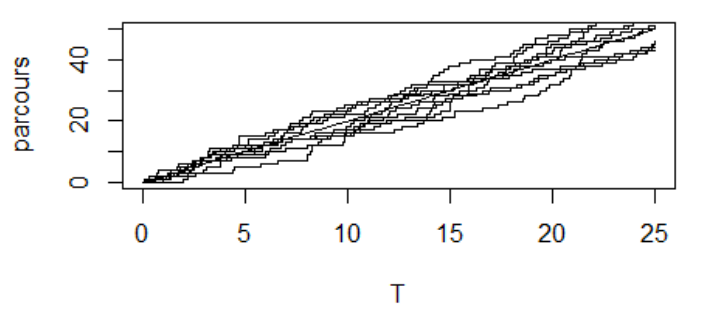
\includegraphics[scale=0.5]{src/TheorieDuRisque/SimulationProcessusPoisson.png}
    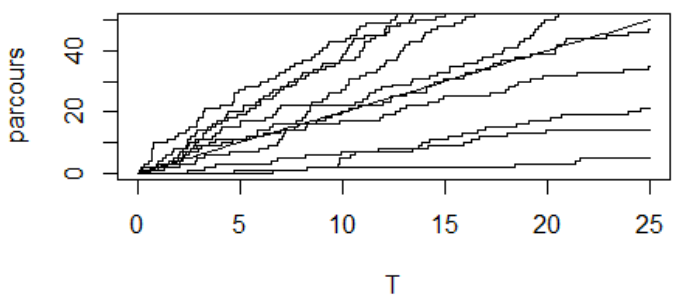
\includegraphics[scale=0.5]{src/TheorieDuRisque/SimulationProcessusPoissonMixte.png}
    \caption{Comparaison entre un processus de Poisson homogène et un processus de poisson mixte. Le graphique du bas représente le processus mixte.}
\end{figure}

\begin{align*}
    \prob{N(t) = n} &= \int_{-\infty}^\infty \prob{N(t) = n | \Lambda} \cdot f_\Lambda(\lambda)\: d\lambda \\ 
    &\text{si } \Lambda \sim \Gamma(\alpha, \beta) \\
    &= \frac{\Gamma(\alpha+n)}{\Gamma(\alpha)k!} \left( \frac{\beta}{\beta + t} \right)^\alpha \left( \frac{1}{\beta + t} \right)^n \sim \text{BinNeg}(\alpha, \frac{\beta}{\beta + t})
\\
    \prob{N(t, t+s] = n} &= \int_{-\infty}^\infty \prob{N(t, t+s] = n | \Lambda} \cdot f_\Lambda(\lambda)\: d\lambda \\
    &= \int_{-\infty}^\infty \prob{N(s) = n | \Lambda} \cdot f_\Lambda(\lambda)\: d\lambda 
\\ \\
    \prob{N(t) = k_1, N(t, t+s] = k_2} &= \int_{-\infty}^\infty \prob{N(t) = k_1, N(t, t+s] = k_2| \Lambda} \cdot f_\Lambda(\lambda)\: d\lambda \\
    &= \int_{-\infty}^\infty \prob{N(t) = k_1 | \Lambda} \prob{N(s) = k_2 | \Lambda}\cdot f_\Lambda(\lambda)\: d\lambda
\end{align*}
\begin{align*}
    \esp{N(t+s)|N(t) = k_1} &= \esp{N(t) + N(t, t+s] | N(t) = k_1} \\
    &= k_1 + \esp[\Lambda]{\esp{N(t, t+s]|N(t) = k_1, \Lambda}|N(t) = k_1} \\
    &= k_1 + \esp[\Lambda]{\lambda t|N(t) = k_1} \\
    &= k_1 + \int_{-\infty}^\infty \lambda t \frac{f_{\Lambda, N(t)}(\lambda, k_1)}{\prob{N(t) = k_1}}\: d\lambda \\
    &= k_1 + \frac{\int_{-\infty}^\infty\lambda t \prob{N(t) = k_1|\Lambda} f_\Lambda(\lambda)\:d\lambda}{\int_{-\infty}^\infty \prob{N(t) = k_1|\Lambda} f_\Lambda(\lambda)\:d\lambda} \\
    &\text{si } \Lambda \sim \Gamma(\alpha, \beta) \\
    &= k_1 + \frac{\alpha + n}{\beta + t}
\end{align*}
\begin{align*}
    F_{W_1}(t) &= \int_{-\infty}^\infty F_{w_1|\Lambda}(t) f_\Lambda(\lambda)\,d\lambda \\
    &\text{si } \Lambda \sim \Gamma(\alpha, \beta) \\
    &= \left( \frac{\beta}{\beta + t} \right)^\alpha \sim \text{Pareto}(\alpha, \beta)
\\ \\
    F_{W_1, W_2}(t_1, t_2) &= \int_{-\infty}^\infty F_{W_1}(t_1) F_{W_2}(t_2) f_\Lambda(\lambda)\,d\lambda\\
    &\text{si } \Lambda \sim \Gamma(\alpha, \beta) \\
    &= \left( \frac{\beta}{\beta + t_1 + t_2 } \right)^\alpha \sim \text{Pareto Mulivarié}
\end{align*}

\label{Chapter:TheorieDuRisque}


% EXAMENS PROFESSIONNELS
\part{Matière pour les examens professionnels}

{ \color{red} This section resume the Chapters 1-5 (excluding Sections 3.3 and 3.4), 6, 7 (Sections 7.1, 7.2 and 7.3) of \emph{An Introductory Time Series with R} }

\hl{A mettre dans la bio: Cowpertwait, P. and Metcalfe, A., Introductory Time Series with R, Springer, 2009.}

\paragraph{Trend}
In general, a systematic change in a time series that does not appear to be periodic is known as a trend.

\paragraph{Seasonal Variation}
A repeating pattern within any fixed period.

\paragraph{Notation}
We represent a time series of length n by ${x_t : t = 1,...,n} = {x_1, x_2, ..., x_n}$

\paragraph{Forecast}
A forecast $\hat{x}_{t+k|t}$ is a predicted future value, and the number of time steps into the future is the \textbf{lead time (k)}

\section{Base Models}

\paragraph{Additive Decomposition}
The additive decomposition model is given by
\[ x_t = m_t + s_t + z_t \]
where $t$ is the time, $x_t$ the observed series, $m_t$ the trend, $s_t$ the seasonal effect and $z_t$ the error term.

\paragraph{Multiplication Model}
If the seasonal effect tends to increase as the trend inscrease, we use a multiplication model define as
\[ x_t = m_t \cdot s_t + z_t \]
where $t$ is the time, $x_t$ the observed series, $m_t$ the trend, $s_t$ the seasonal effect and $z_t$ the error term.

\subsection{Estimating Trends}

\paragraph{Centered Moving Average}
A moving average is an average of a specified number of time series values around each value in the time series, with the exception of the first few and last few terms.
The length of the moving average is chosen to average out the seasonal effects, which can be estimated
\[ \hat{m}_t = \frac{0.5m_{t-k} + m_{t-k-1} + ... + m_t + ... + m_{t+k-1} + 0.5m_{t+k}}{2k} \]

\subsection{Estimating Seasonal Effect}

\paragraph{Additive Effect}
An estimate of the monthly additive effect ($s_t$) at time t is define by
\[ \hat{s}_t = x_t - \hat{m}_t \]
It is usual to adjust those estimate in order that the sum of one period of the time serie equal zero. Let $c$ be that adjustment in order to solve this expression.
\[ \sum (s_t + c) = 0 \]

\paragraph{Multiplicative Effect}
An estimate of the monthly multiplicative effect ($s_t$) at time t is define by
\[ \hat{s}_t = \frac{x_t}{\hat{m}_t} \]
And we found the ajustment $c$ in order to solve this expression.
\[ \sum \frac{(\hat{s}_t + c)}{n} = 1 \] 

\begin{figure}[!ht]
    \centering 
    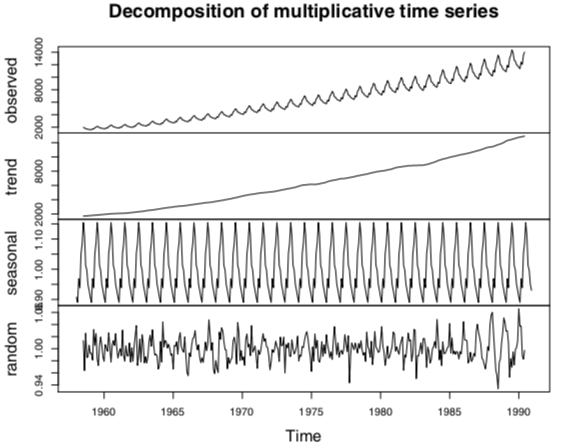
\includegraphics[scale=0.6]{src/SerieChronologique/DecompositionMultiTimeSerie.png}
    \caption{In this example, the multiplicative model would seem more appropriate than the additive model because the variance of the original series and trend increase with time} 
\end{figure}

\subsection{Smoothing Procedure}
Smoothing procedures can, and usually do, use points before and after the time at which the smoothed estimate is to be calculated. A consequence is that the smoothed series will have some points missing at the beginning and the end unless the smoothing algorithm is adapted for the end points.
\begin{itemize}
    \item[Ex.1] The centering moving average is an exemple of a \emph{smoothing} procedure. 
    \item[Ex.2] The \emph{loess} technique is also a \emph{smoothing} that use a locally weighted regression.

\end{itemize}

\section{Correlation}

\paragraph{Mean Function}
The mean function is, in general, a function of t and it define as 
\[\mu(t) = \esp{x_t} \]

\paragraph{Sample Mean}
The sample mains is define as
\[ \bar{x} = \sum \frac{x_i}{n} \]

\paragraph{Variance Function}
The variance function of a time series model that is stationary in the mean is
\[ \sigma^2(t) = \esp{(x_t - \mu^2)} \]

\paragraph{Sample Variance}
If the model is stationary in the variance, we can estimate the variance with the sample variance define as
\[ \variance{x} = \frac{\sum (x_t - \bar{x}}{n-1} \]

\paragraph{Stationarity}
If the mean function is constant, we say that the time series model is stationary in the mean. The time serie can also be stationary in the variance, if the variance function is constant $\sigma^2$.

\paragraph{Ergodic Serie}
A time series model that is stationary in the mean is ergodic in the mean if the time average for a single time series tends to the ensemble mean as the length of the time series increases.
\[ \lim_{n \to \infty} \bar{x} = \mu \]

\paragraph{Covariance}
The covariance measure the \emph{linear association} between two random variables. The covariance is define as
\[ \gamma(x,y) = \esp{(x - \mu_x)(y - \mu_y)} \]

\paragraph{Sample Covariance}
We can estimate the covariance with the sample covariance define as
\[ \covar{x, y} = \sum \frac{(x_i - \bar{x})(y_i - \bar{y})}{n-1} \]

\paragraph{Correlation}
Correlation is a dimensionless measure of the linear association between a pair of variables (x,y) and is obtained by standardising the covariance.
\[ \rho(x, y) = \frac{\esp{(x-\mu_x)(y-\mu_y)}}{\sigma_x \sigma_y} = \frac{\gamma(x,y)}{\sigma_x \sigma_y} \]
 
\paragraph{Sample Correlation}
We can estimate the covariance with the sample covariance define as
\[ \mathrm{Cor}(x, y) = \frac{\covar{x, y}}{\mathrm{sd}(x)\mathrm{sd}(y)} \]

\paragraph{Autocovariance (acvf)}
If a time series model is second-order stationary, we can define an autocovariance function (acvf), $\gamma_k$ , as a function of the lag $k$.
\[ \gamma_k = \esp{(x_t-\mu)(x_{t+k}-\mu)} \]

\paragraph{Sample Autocorrelation}
The acvf function can be estimated by
\[ c_k = \frac{1}{n} \sum_{t=1}^{n-k} (x_t - \bar{x})(x_{t+k} - \bar{x}) \]

\begin{note}
The sample autocovariance at lag 0, $c_0$, is the variance calculated with a denominator $n$. 
\end{note}

\paragraph{Autocorrelation (acf)}
The lag $k$ autocorrelaton function (acf), $\rho_k$, is defined by
\[ \rho_k = \frac{\gamma_k}{\sigma^2} \]
where $\rho_0 = 1$

\paragraph{Sample Autocorrelation}
The acf function can be estimated by
\[ r_k = \frac{c_k}{c_0} \]

\paragraph{Second-order Stationary}
Suppose a the time serie that is stationary in the mean and the variance. Then, the time serie model is second-order stationary if the correlation between variable depends only on the number of time steps separating them.


\subsection{The Correlogram}
The correlogram is plot of $r_k$ against k. The main use of the correlogram is to detect autocorrelations in the time series after we have removed an estimate of the trend and seasonal variation.

\begin{itemize}
    \item[\textbullet] The x-axis gives the lag ($k$) and the y-axis gives the autocorrelation ($\rho_k$) at each lag. The unit of lag is the sampling interval. Correlation is dimensionless, so there is no unit for the y-axis.
    \item[\textbullet] The dotted lines on the correlogram are drawn at 
        \[ -\frac{1}{n} \pm \frac{2}{\sqrt{n}} \]
    \item[] If the sample acf($r_k$) falls outside these line, we have evidence against the null hypothesis that $p_k = 0$ at the 5\% level.
    \item[\textbullet] The lag at 0 is always.
\end{itemize}

\begin{figure}[!ht]
    \centering 
    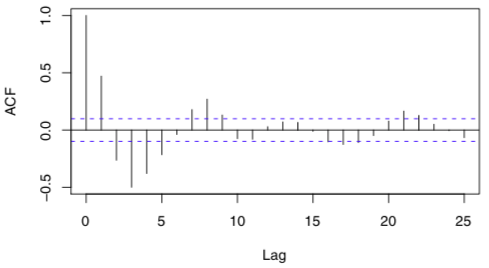
\includegraphics[scale=0.7]{src/SerieChronologique/Correlogram.png}
    \caption{Correlogram}
\end{figure}


\subsection{Covariance of sums of random variables}
Let $x_1, x_2,...,x_n$ and $y_1, y_2,..., y_m$ be random variables. Then 
\[ \covar{\sum_{i=1}^{n} x_i, \sum_{j=1}^{m}} y_j = \sum_{i=1}^{n} \sum_{j=1}^{m} \covar{x_i, y_i} \]
The result tells us that the covariance of two sums of variables is the sum of all possible covariance pairs of the variables.

\section{Forecasting Strategies}

\subsection{Relationships of different time serie}

\paragraph{Cross-covariance (ccvf)}
The cross-correlation (ccvf) between two time series is define as
\[ \gamma_k(x, y) = \esp{(x_{t+k} - \mu_x)(y_t - \mu_y)} \]

\begin{note}
    This is not a symmetric relationship, and the variable $x$ is lagging variable $y$ by $k$.
    \[\gamma_k(x, y) = \gamma_{-k}(y, x) \]
\end{note}

\paragraph{Sample Cross-covariance}
The ccvf function can be estimed by
\[ c_k(x, y) = \frac{1}{n} \sum_{t=1}^{n-k} (x_{t+k} - \bar{x})(y_k - \bar{y}) \]

\paragraph{Cross-correlation (ccf)}
The cross-correlation (ccf) between two time serie is define as 
\[ /rho_k(x, y) = \frac{\gamma_k(x, y)}{\sigma_x\sigma_y} \]

\begin{note}
    This is not a symmetric relationship, and the variable $x$ is lagging variable $y$ by $k$.
    \[\rho(x, y) = \rho_{-k}(y, x) \]
\end{note}

\paragraph{Sample Cross-correlation}
The ccf function can be estimed by
\[ r_k(x, y) = \frac{c_k(x, y)}{\sqrt{c_0(x, x) x_0(y, y)}} \]

\section{Basic Stochastic Models}

We may consider a \textbf{trend} to be \textbf{stochastic} when it shows inexplicable changes in direction. Those type of trend can be simulated by the models of this section.

\subsection{White Noise}

\paragraph{Residual Error}
A residual error is the difference between the observed value and the model predicted value at time t. Then the residual error, $x_t$, is defined by
\[ x_t = y_t - \hat{y}_t \]
where $y_t$ is the observed value and $\hat{y_t}$ the predicted value.

As the residual errors occur in time, they form a time series: $x_1, x_2,..., x_n$.

\paragraph{Definition} 
A white noise is a time serie $\{w_t : t = 1,2,...,n\}$ where each term is independent and with a constant variance $\sigma^2$.
\[ w_t \sim \mathrm{N}(0, \sigma^2) \]

\begin{figure}[!ht]
    \centering
    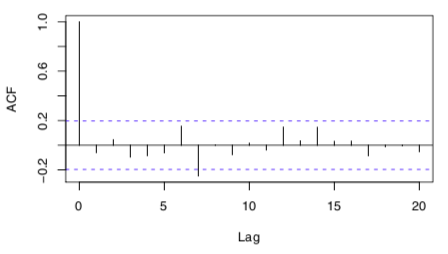
\includegraphics[scale=0.7]{src/SerieChronologique/WhiteNoise-Correlogram.png}
    \caption{Correlogram of a simulated white noise series. The underlying autocorre- lations are all zero (except at lag 0); the statistically significant value at lag 7 is due to sampling variation.}
\end{figure}

\subsection{Random Walks}

\paragraph{Definition}
Let $\{x_t\}$ be a time series. Then $\{x_t\}$ is a random walk if 
\[ x_t = x_{t-1} + w_t \]
where $\{w_t\}$ is a white noise.

\paragraph{Backward Operator}
The backward operator(or lag operator)  $\mathbf{B}$ is defined by
\[ \mathbf{B}^n = x_{t-n} \]

\paragraph{Second-order Properties}
The covariance is in function of time, so a random walk is non-stationary. This model is only suitable for short term predictions.
\begin{align*}
        \hspace*{1cm}
      \mu(t) &= 0 \\
      \sigma^2(t) &= t\sigma_w^2 \\
      \gamma_k(t) &= t\sigma_w^2 \\
      \rho_k(t) &= \frac{1}{\sqrt{1 + \frac{k}{t}}}
\end{align*} 

\paragraph{The Difference Operator}
The defference operator is defined by
\[ \nabla x_t = x_t - x_{t-1} \] 
We can also expresse it with the Backward operator
\[ \nabla^n x_t  = (1 - \mathbf{B})^n x_t \]
\begin{note}
Differencing adjacent terms of a series can transform a non-stationary series to a stationary series.
    \[ x_t - x_{t-1} = w_t \]
Here differencing two non-stationary random walk give a stationary white noise.
\end{note}

\begin{figure}[!ht]
    \centering
    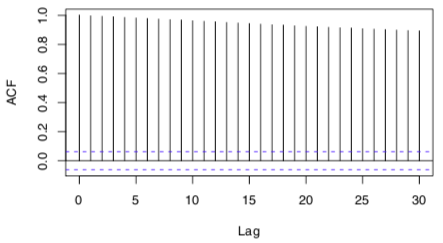
\includegraphics[scale=0.7]{src/SerieChronologique/RandomWalk-Correlogram.png}
    \caption{The correlogram for the simulated random walk. A gradual decay from a high serial correlation is a notable feature of a random walk series.}
\end{figure}

\paragraph{Random Walk with Drift}
A Random walk with drif is a random walk with a mean. it defined as
\[ x_t = \delta + x_{x-1} + w_t \] 

\subsection{Autoregressive Models}

\paragraph{Definition}
The series $\{xt\}$ is an autoregressive process of order p, abbreviated to $\mathrm{AR(p)}$, if
\[ x_t = \alpha_1 x_{t-1} + \alpha_2 x_{x-2} + ... + \alpha_p x_{t-p} + w_t \] 
where $\alpha_i$ are the model parameters with $\alpha_p \neq 0$.

The following points should be noted:
\begin{itemize} 
    \item[\textbullet] The random walk is a special case of $\mathrm{AR(1)}$ with $\alpha_1 = 1$.
    \item[\textbullet] The model is a regression of $x_t$ on past terms from the same series, that where the name \emph{autoregressive} come.
    \item[\textbullet] A prediction at time $t$ is given by
        \[ \hat{x}_t = x_t = \alpha_1 x_{t-1} + \alpha_2 x_{x-2} + ... + \alpha_p x_{t-p} \]
    \item[\textbullet] The model parameters can be estimated by minimising the sum of squared errores.
\end{itemize}

\paragraph{Stationary and non-stationary AR processes}
We can expressed a AR model as a polynomial of order p in terms of the backward shift operator
\[ \theta_p(\mathrm{B})x_t = (1 - \alpha_1\mathrm{B} - \alpha_2 \mathrm{B}^2 - ... - \alpha_p \mathrm{B}^p)x_t = w_t \]
Then a AR model is stationary if all root of $\theta_p(\mathrm{B})$ exceed one in absolute values. In other word if 
\begin{center}
if all $|\mathrm{B_i}| > 1$ then the model is stationary \\
otherwise, the model is non-stationary
\end{center}

\paragraph{Second-order properties of an AR(1) model}
    \begin{align*}
      \mu_k &= 0 \\  
      \gamma_k &= \frac{\alpha^k \sigma_w^2}{1 - \alpha^2} \\
      \rho &= \alpha^k
\end{align*}

\begin{figure}[!ht]
    \centering
    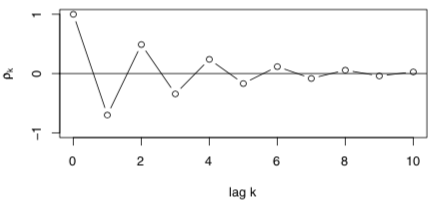
\includegraphics[scale=0.7]{src/SerieChronologique/AR-Correlogram.png}
    \caption{For an AR model, the correlograms decays to zero. The correlogram decays to zero more rapidly for small $\alpha$.}
\end{figure}

\paragraph{Partial Autocorrelation}
An AR(p) process has a correlogram of partial autocorrelation $\alpha_k$ that is zero after lag p.

\section{Regression}

When we have some plausible physical explanation for a \textbf{trend} we will usually wish to model it in some \textbf{deterministic} manner. Therefore, the model of this section can be used.
\\
\\
The difference with \textbf{deterministics trend} is the when we make short term forecast, we assume that the trend will change slowly.
\\
\\
Time series regression usually differs from a standart regression analysis because the residual form a time serie and therefore tend to be serially correlated. When this correlation is possitive, the estimated standard errors of the parameter estimates, read from the computer output of a standard re- gression analysis, will tend to be less than their true value.

\subsection{Linear Models}

\paragraph{Definition}
A model for a time series $\{ x_t : t = 1,...,n\}$ is linear if it can be expressed as
\[ x_t = \alpha_0 + \alpha_1 u_{1,t} + \alpha_2 u_{2,t} + ... + \alpha_m u_{m,t} + z_t \]
where $u_{i,t}$ is the value of the i\up{th} explanatory variable, $\alpha_i$ the estimated model parameters, $z_t$ the error at time $t$.

An example of a linear model is the pth-order polynomial function of t:
\[ x_t = \alpha_0 + \alpha_1 t + \alpha_2 t^2 + ... + \alpha_p t^p + z_t \]

\begin{note} 
    Note that the errors form a time series $\{z_t\}$, with mean 0, that does not have to be Gaussian or white noise.
\end{note} 

\paragraph{Stationarity}
Linear models for time series are non-stationary when they include functions of time.

Differencing can remove both stochastic and deterministic trends from time series. Then for a polynomial of roder $m$, the mth-order differencing is required to remove the trend.
\paragraph{Autocorrelation variance estimation of the sample mean}
Let $\{x_t : t = 1,..., n\}$ be a stationary time serie with mean $\mu$, variance $\sigma^2$ and autocovariance $\covar{x_t, x_{t+k}}$. Then the variance of the sample mean is given by
\[ \variance{\bar{x}} = \frac{\sigma^2}{n} \left[ 1 + 2 \sum_{k=1}^{n-1} (1 - \frac{k}{n}) \rho_k \right] \] 

\paragraph{Generalised least squares}
A fitting procedure known as generalised least squares (GLS) can be used to provide better estimates of the standard errors of the regression parameters to account for the autocorrelation in the residual series.

\subsection{Linear Models with Seasonal Variables}

\paragraph{Additive Seasonal Indicator Variables}
To include seasonal effect, we change the constant $\alpha_o$ depending on the season. Let $s$ be the time serie measured (Ex. for monthly time serie, $s=12$). Then for each $s$, we fit a constant term.
\[ x_t = s_t + m_t + z_t \]
where $s_t$ is the seasonal constant when t falls in the i\up{th} season, $m_t$ a linear model for the trend and $z_t$ the error term.

\paragraph{Harmonic Seasonal models}
The advantage of this model is that we can represente the seasonal effect with something that is smoothly. For a time series $\{x_t\}$ with $s$ season, there are $\lfloor s/2 \rfloor$ possible cycles. The harmonic model is defined by 
\[ x_t = m_t + \sum_{i=1}^{\lfloor s/2 \rfloor} \left\{ s_i \sin(\frac{2\pi it}{s}) + c_i \cos(\frac{2\pi it}{s}) \right\} + z_t \]
where $m_t$ is a trend model \textbf{that include a constant term} ($\alpha_0$) and $s_i$ and $c_i$ are unknown parameters. 

\begin{figure}[!ht]
    \centering 
    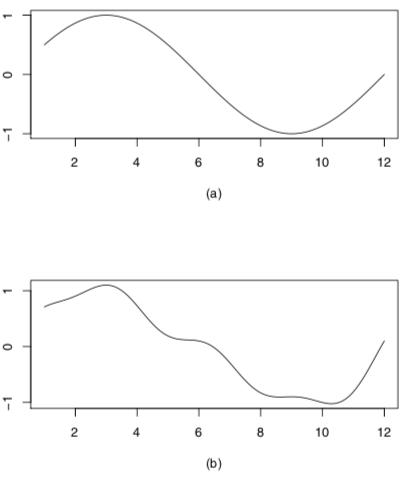
\includegraphics[scale=0.7]{src/SerieChronologique/HarmonicModel.png}
    \caption{Two possible underlying seasonal patterns for monthly series based on the harmonic model (Equation (5.10)). Plot (a) is of the first harmonic over a year and is usually too regular for most practical applications. Plot (b) is of the same wave but with a further two harmonics added. Plot (b) illustrates just one of many ways that an underlying sine wave can be perturbed to produce a less regular, but still dominant, seasonal pattern of period 12 months.}
\end{figure}

\subsection{Forecasting from regression}
When we predic a regression time series, we try to predict in the future. The problem is that the trend might change. Therefore, it is better ot think of a forecast from a regression model as an expected value conditional on past trends continuing into the future.

\paragraph{Bias Correction} 
The process of transforming the model introduce some bias in the mean. We need to apply a correction to the mean. Note that this correction doesn't need to be apply in simulation.
\[ \hat{x}_t' = \hat{x}_t * \text{Correction} \]

\subparagraph{Lognormal Correction}
\[ e^{\sigma^2 /2} \]
\subparagraph{Empirical Correction}
\[ \frac{1}{n} \sum e^{z_t} \]

\section{Stationary Models}
Sometime, the residual will be correlated in time, as this is not accounted in the fitted regression model, we need other model. 

\subsection{Strictly Stationary Series}
A time series model $\{ x_t \}$ is \emph{strictly stationry} if the joint statistical distribution $x_{t_1},...,x_{t_n}$ is the same as the joint distribution of $x_{t_1 + m},...,x_{t_n + m}$ for all $t_1, ..., t_n$ and $m$, so that the distribution is unchanged after an arbitrary time shift.

\begin{note}
    Note that strict stationarity implies that the mean and variance are constant in time and that the autocovariance $ \covar{x_t, x_s} = \gamma_k$ (i.e. only depend on the lag $k$). If a series is not strictly stationary but the mean and variance are constant in time and the autocovariance only depends on the lag, then the series is called \emph{second-order stationary}.
\end{note}
We focus on the second-order properties in this chapter, but the stochastic processes discussed are strictly stationary.
\\ 
\\
Stationarity is an idealisation that is a property of models. If we fit a stationary model to data, we assume our data are a realisation of a stationary process. So our first step in an analysis should be to check whether there is any evidence of a trend or seasonal effects and, if there is, remove them. Regression can break down a non-stationary series to a trend, seasonal components, and residual series. It is often reasonable to treat the time series of residuals as a realisation of a stationary error series. Therefore, the models in this chapter are often fitted to residual series arising from regression analyses.

\subsection{Moving average models}

\paragraph{Definition}
 moving average (MA) process of order q is a linear combination of the current white noise term and the q most recent past white noise terms and is defined by
\[ x_t = w_t + \beta_1 w_{t-1} + ... + \beta_q w_{t-q} = \phi_q(\mathrm{B}) w_t \]
where $\phi_q$ is a polynomial of order q. Because MA processes consist of a finite sum of stationary white noise terms, they are stationary and hence have a time-invariant mean and autocovariance.

\paragraph{Second-order properties}
\begin{align*}
    \mu &= 0 \\
    \sigma^2 &= \sigma_w^2 (1 + \beta_1^2 + ... + \beta_q^2) \\
    \gamma_k &= \sigma_w^2 \sum_{i=0}^{q-k} \beta_i \beta_{i+k} \\
    \rho_k &= \frac{\sum_{i=0}^{q-k} \beta_i \beta_{i+k}}{\sum_{i=0}{q} \beta_i^2 }
\end{align*}

\paragraph{Invertible properties}
An MA process is invertible if it can be expressed as a stationary AR($\infty$) process of infinite order without an error term.
\[ w_t = (1 - \beta \mathrm{B})^{-1} x_t = x_t + \beta x_{t-1} + \beta^2 x_{t-2} + ... \]
provided $|\beta| < 1$, which is required for convergence.

\begin{figure}[!ht]
    \centering
    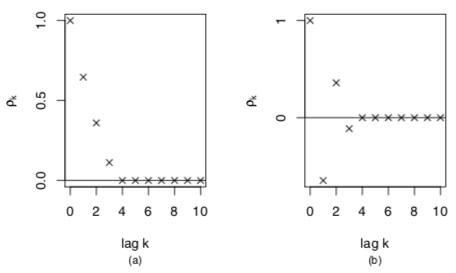
\includegraphics[scale=0.7]{src/SerieChronologique/MA-Correlogram.png}
    \caption{Plots of the autocorrelation functions for two MA(3) processes. The autocorrelation for lag $k>q$ are all zero. $(a) \beta_1 = 0.7, \beta_2 = 0.5, \beta_3 = 0.2; (b) \beta_1 = -0.7, \beta_2 = 0.5, \beta_3 = -0.2$.}
\end{figure}

\subsection{Mized Models: The ARMA process}

\paragraph{Definition}
The ARMA model is a AR(p) + MA(q) models defined as
\[ x_t = \alpha_1 x_{t-1} + \alpha_2 x_{t-2} + ... + \alpha_p x_{t-p} + w_t + \beta_1 w_{t-1} + \beta_2 w_{t-2} + ... + \beta_q w_{t-q} \]
We can also express it as 
\[ \theta_p(\mathrm{B}) x_t = \phi_q(\mathrm{B}) w_t \]
\begin{itemize}
    \item[\textbullet] The process is stationary when the roots of $\theta$ are all exceed unity in absolute value.
    \item[\textbullet] The process is invertible when the roots of $\phi$ all exceed unity in absolute value.
    \item[\textbullet] The AR(p) model is the special case ARMA(p, 0).
    \item[\textbullet] The MA(q) model is the special case ARMA(0, q).
    \item[\textbullet] \textbf{Parameter parsimony.} When fitting to data, an ARMA model will often be more parameter efficient (i.e., require fewer parameters) than a single MA or AR model.
    \item[\textbullet] \textbf{Parameter redundancy.} When $\theta$ and $\phi$ share a common factor, a stationary model can be simplified. For example, the model:
        \begin{align*}
            (1 - \frac{1}{2}B)(1 - \frac{1}{3}B)x_t &= (1 - frac{1}{2}B)w_t \\
            (1 - \frac{1}{3}B)x_t &= w_t
        \end{align*}
\end{itemize}

\paragraph{Second-order Properties}
\begin{align*}
    \sigma^2 &= \sigma_w^2 \left( 1 + \frac{(\alpha+\beta)^2}{1 - \alpha^2} \right) \\
    \gamma_0 &= \sigma_w^2 \left( \frac{1 + 2 \alpha \beta + \beta^2}{1 - \alpha^2} \right) \\
    \gamma_k &= \sigma_w^2 (\alpha + \beta)\alpha^{k-1} \left( \frac{1 + \alpha \beta}{1 - \alpha^2} \right) \\
    \rho_k &= \frac{\alpha^{k-1}(\alpha+\beta)(1+\alpha\beta)}{1 + \alpha\beta + \beta^2} = \alpha \rho_{k-1}
\end{align*}

\section{Non-stationary Models}

\subsection{Differencing}
Differencing a serie $\{x_t\}$ can remove trends, whether these trend are stochastic, as in a random walk, or deterministic, as in the case of a linear trend. 

\subparagraph{Differencing random walk}
\[ \nabla x_t = x_t - x_{t-1} = w_t \]
which is a stationary white noise.

\subparagraph{Differencing linear trend}
\[ \nabla x_t = x_t - x_{t-1} = b + w_t - w_{t-1} \]
which is a stationary moving average process rather than white noise.

\paragraph{Integrated Model}
A serie $\{x_t\}$ is integrated of order d, $I(d)$, if the d\up{th} difference of $\{x_t\}$ is a white noise
\[ (1 - \mathrm{B})^d x_t = w_t \]

\begin{note}
    The random walk is a special case $I(1)$
\end{note}

\subsection{Non-Seasonal ARIMA Models}

\paragraph{Definition}
A time series $\{x_t\}$ follows an ARIMA($p, d, q$) process id the d\up{th} differences of the $\{x_t\}$ series are an ARIMA($p, q$) process
\[ \theta_p(\mathrm{B}(1 - \mathrm{B})^d x_t = \phi_q(\mathrm{B}) w_t \]

In general:
\begin{itemize}
    \item[\textbullet] $\text{ARIMA}(0,d,q) \equiv \text{IMA}(d, q)$
    \item[\textbullet] $\text{ARIMA}(p,d,0) \equiv \text{ARI}(p,d)$
\end{itemize}

\subsection{Seasonal ARIMA models}
A seasonal ARIMA model uses differencing at a lag equal to the number of seasons (s) to remove additive seasonal effects. As with lag 1 differencing to remove a trend, the lag s differencing introduces a moving average term.
\\
\\
The ARIMA$(p,d,q)(P,D,Q)_s$ model can be defined as
\[ \Theta_P(\mathrm{B}^s)\theta_p(\mathrm{ B})(1 - \mathrm{B}^s)^D (1 - \mathrm{B})^d x_t = \Phi_Q(\mathrm{B}^s) \phi_q(\mathrm{B}) w_t \]


\label{Chapter:SerieChronologique}

\chapter{Extended Linear Models}
\chapter{Extended Linear Models}

{ \color{red} Thissection resume the Chapters 5-9 of \emph{An Introduction to Generalized Linear Models}.}

\hl{Add to biblio:}

\section{Inference}

The two tool to do inference are \textbf{confidence intervals} and \textbf{hypothesis tests}. For GLM, a hypothesis tests can be use to compare two models, but their need to have the same probability function and the same link. Also, the null hypothesis $H_0$ is a sinpler model and must be a special case of the other. 

\subsection{Sampling distribution for the score statistic}
\paragraph{Score Function}
Let $\ell = \ln f(y)$ be the log-likehood function, then the score function $U$, is define as
\[ U_j = \frac{\partial \ell}{\partial \mu} = \sum_{i=1}^N \left[ \frac{(Y_i - \mu_i)}{\variance{Y_i}} x_{i,j} \left( \frac{\partial \mu_i}{\partial \eta} \right) \right] \]

\paragraph{Information matrix}
The information matrix is define as the variance-covariance matrix of the score function. This information matrix is defined as 
\[ I(\theta) = \variance{U} \]

\paragraph{Score Statistic}
If there is only one $\beta$, the score statistic has the asymptotic sampling distribution
\[ \frac{U}{\sqrt{I(\theta)}} \sim N(0, 1),  \frac{U^2}{I(\theta)} \sim \chi^2(1) \]

If there is a vector of $\underline{\beta}$
\[ U^T I(\theta)^{-1} U \sum \chi^2(p) \]

\section{Normal Linear Models}
\subsection{Basis Result}

\paragraph{Maximum likelihood}
The maximum likelihood estimation of $\beta$ is given by
\[ \mathrm{b} = (\mathrm{X}^T \mathrm{X})^{-1} \mathrm{X}^T \mathrm{y} \]
The estimator is unbiasedm with the variance-covariance matrix
\[ I(\theta)^{-1} = \sigma^2 (\mathrm{X}^T \mathrm{X}^{-1}) \]
However, the unbiased estimator of $\sigma^2$ is given by
\[ \hat{\sigma^2} = \frac{1}{N-p} (\mathrm{y} - \mathrm{X}\mathrm{b})^T \]

\paragraph{Least Square Estimation}
In the case of linear models, we obtain the same result as the maximum likelihood
\[ \mathrm{b} = (\mathrm{X}^T \mathrm{X})^{-1} \mathrm{X}^T \mathrm{y} \]

\paragraph{Deviance}
The diviance is define by the square of the error $\mathrm{\varepsilon}$.
\[ \frac{1}{\sigma^2} \mathrm{\varepsilon}^T \mathrm{\varepsilon} = \frac{1}{\sigma^2} (\mathrm{y} - \mathrm{X}\mathrm{b})^T(\mathrm{y} - \mathrm{X}\mathrm{b}) \]
or, in case of simple linear model,
\[ \frac{1}{\sigma^2} \sum (Y_i - \hat{Y_i})^2 \]


\label{Chapter:ExtendedLinearModels}

% ANNEXES DU DOCUMENT
\appendix
\chapter{Principales distribution de probabilité utilisées}
introduction

% Annexe des preuves
\chapter{Résultats (et démonstrations) utiles}

% \chapter{Preuves}
\section{Stop-Loss ($\pi_X(d)$)}
\label{preuve:stoploss}
Dans un contexte continu,
\begin{align*}
\pi_X(d) = \int_d^\infty \overline{F}(d) du
\end{align*}

\begin{proof}
\begin{align*}
\pi_X(d)		& = E[\max(X-d,0)] \\
	& = \int_0^\infty \max(x - d, 0) F_X(x) dx \\
	& = \int_0^\infty (x-d) 1_{\{X > d \}} f_X(x) dx \\
	& = \int_d^\infty (x-d) f_X(x) dx \\
	& = \int_d^\infty x f_X(x) dx - \int_d^\infty d f_X(x) dx \\
\end{align*}
On doit alors faire une intégration par partie, en posant

\begin{displaymath}
\begin{aligned}
u	& = x		& du	 & = dx \\
dv	& = dF_X(x)	& v	 & = -S(x) \\	
\end{aligned}
\end{displaymath}
Note : si on fait tendre $S(x)$ vers l'infini, ça va tendre plus rapidement vers 0 que $x$ seul.
\begin{align*}
\pi_X(d)	& = -xS(x) \eval_d^\infty - \int_d^\infty - S(x) dx - d \big(F(\infty) - F(d) \big) \\
	& = 0 + \cancel{dS(d)} + \int_d^\infty S(x) dx - \cancel{dS(d)} \\
	& = \int_d^\infty S(x) dx \\
\end{align*}
\end{proof}
Il existe aussi le contexte discret : 
\begin{align*}
\pi_X(d) = \sum_{k=d}^\infty S(k)
\end{align*}
\begin{proof}
\begin{align*}
\pi_X(k) 	& = E[\max(N-k),0)] \\
	& = \sum_{j=k}^\infty (j-k) P(N = j) \\
	& = (k-k) P(N = k) + ((k+1)-k) P(N = k+1) + P((k+2)-k) P(N = k+2) + ... \\
	& = P(N = k+1) + 2 P(N = k+2) + 3 P(N = k+3) + ... \\
	& = \underbrace{(P(N = k+1) + P(N = k+2) + P(N = k+3) + ...)}_{S(k)} \\
	& + \underbrace{(P(N = k+2) + P(N = k+3) + P(N = k+4) + ...)}_{S(k+1)} \\
	& + \underbrace{(P(N = k+3) + (PN = k+4) + P(N = k+5) + ...)}_{S(k+2)} \\
	& + ... \\
	& = \sum_{i = k}^\infty S(i)
\end{align*}
\end{proof}

\section{TVaR}
\subsection{Les 3 formes explicites de la $TVaR$	}
\label{sec:preuve}

Pour la $TVaR$, il y a 3 preuves à bien connaître : 
\begin{equation*}
TVaR_\kappa(X) = \frac{1}{1 - \kappa} \pi_X(VaR_\kappa(X)) + VaR_\kappa(X)
\end{equation*}


\begin{proof}
\label{preuve:tvar_stoploss}
\begin{align*}
TvaR_\kappa(X)  & = \frac{1}{1 - \kappa} \int_\kappa^1 VaR_u(X) du \\
    & = \frac{1}{1 - \kappa} \int_\kappa^1 (VaR_u(X) - VaR_\kappa(X) + VaR_\kappa(X)) du \\
    & = \frac{1}{1 - \kappa} \int_\kappa^1 (\underbrace{VaR_u(X)}_{\substack{\text{fonction} \\ \text{quantile}}} - VaR_\kappa(X)) du + \underbrace{\int_\kappa^1 VaR_\kappa(X) du}_{\text{intégration d'une constante}} \\
    & = \frac{1}{1 - \kappa} \int_\kappa^1 (F_X^{-1}(u) - VaR_\kappa(X)) \underbrace{f_U(u)}_{U \backsim Unif(0,1)} du + \frac{1}{\cancel{1 - \kappa}} VaR_\kappa(X) (\cancel{1 - \kappa}) \\
    & = \frac{1}{1 - \kappa} E[\max(\underbrace{F_X^{-1}(U)}_{F_X^{-1} \backsim X} - VaR_\kappa(X);0)] + VaR_\kappa(X) \\
    & = \frac{1}{1 - \kappa} E[\max(X - VaR_\kappa(X) ; 0)] + VaR_\kappa(X) \\
    & = \frac{1}{1 - \kappa} \pi_X(VaR_\kappa(X)) + VaR_\kappa(X) \\
\end{align*}
\end{proof}

à partir de la preuve ci-dessus, on peut démontrer celle-ci : 
$$
TVaR_\kappa(X) = \frac{E[X \times 1_{\{X > VaR_\kappa(X) \}}] + VaR_\kappa(X)(F_X(VaR_\kappa(X)) - \kappa)}{1-\kappa} 
$$

\begin{proof}
\begin{align*}
TVaR_\kappa(X)  & = \frac{1}{1 - \kappa} \pi_X(VaR_\kappa(X)) + VaR_\kappa(X) \\
    & = \frac{1}{1 - \kappa} E[\max(X - VaR_\kappa(X); 0)] + VaR_\kappa(X) \\
    & = \frac{1}{1 - \kappa} E[(X - VaR_\kappa(X)) \times 1_{\{X > VaR_\kappa(X) \}}] + VaR_\kappa(X) \\
    & = \frac{1}{1 - \kappa} E[X \times 1_{\{X > VaR_\kappa(X) \}}] - \frac{1}{1 - \kappa} E[VaR_\kappa(X) \times \underbrace{1_{\{X > VaR_\kappa(X) \}}}_{= S_X(VaR_\kappa(X))}] + VaR_\kappa(X) \\
    & = \frac{1}{1 - \kappa} E[X \times 1_{\{X > VaR_\kappa(X) \}}] - \frac{1}{1 - \kappa} VaR_\kappa(X)(1 - F_X(VaR_\kappa(X))) + \frac{1 - \kappa}{1 - \kappa}VaR_\kappa(X) \\
    & = \frac{E[X \times 1_{\{X > VaR_\kappa(X) \}}] + VaR_\kappa(X)(-1 + F_X(VaR_\kappa(X)) + 1 - \kappa)}{1 - \kappa}  \\
    & = \frac{E[X \times 1_{\{X > VaR_\kappa(X) \}}] + VaR_\kappa(X)(F_X(VaR_\kappa(X)) - \kappa)}{1 - \kappa}  \\
\end{align*}
\end{proof}

Une dernière preuve fortement utilisée pour la $TVaR$, qui découle directement de la dernière :  : 
\begin{align*}
TVaR_\kappa(X) = \frac{E[X \times 1_{\{X > VaR_\kappa(X) \}}]}{1 - \kappa}  \\
\end{align*}


\begin{proof}
Étant donné que cette formule ne fonctionne seulement que pour une v.a. continue, elle est très facile à prouver : 
\begin{align*}
\text{si $X$ est continue}, \quad \forall x, F_X(VaR_\kappa(X))) = \kappa \\
\end{align*}
Alors, on peut enlever la partie de droite de l'équation.
\end{proof}

\section{Sous-additivité de la $TVaR$}
\label{preuve:subadditivity_tvar}
Il y a \blue{\href{https://people.math.ethz.ch/~embrecht/ftp/Seven_Proofs.pdf}{plusieurs façons}} de prouver la sous-additivité de la $TVaR$.

\subsection{À l'aide de la fonction convexe $\varphi(x)$}


On sait que la fonction $\varphi(x)$ est convexe : 
\begin{align*}
\varphi(x) = x + \frac{1}{1 - \kappa} \pi_X(x)
\end{align*}

Et on sait aussi que 
\begin{align*}
TVaR_\kappa(X) = \inf \big \{ \varphi(x) \big \}
\end{align*}

Il faut prouver que $TVaR_\kappa(X + Y) \le TVaR_\kappa(X) + TVaR_\kappa(Y)$
\begin{proof}
Puisque $\varphi(x)$ est une fonction convexe, on peut dire que
\begin{align*}
TVaR_\kappa(X) & \le \varphi(x) \\
	& \le x + \frac{1}{1 - \kappa} \pi_X(x) \\ 
\end{align*} 
On pose le changement de variable \fbox{$X^* = \alpha X + (1-\alpha ) Y$}
\p
On peut donc remplacer $x$ dans $\varphi(x)$ par
\begin{align*}
x_0 & = VaR_\kappa(X^*) \\
	& = VaR_\kappa(\alpha X + (1-\alpha ) Y) \\
	& = \alpha VaR_\kappa(X) + (1-\alpha) VaR_\kappa(Y) \\
\end{align*}
Alors,

\begin{align*}
TVaR_\kappa(\alpha X + (1-\alpha ) Y) & \le \alpha VaR_\kappa(X) + (1-\alpha) VaR_\kappa(Y) \\
	& + \frac{1}{1 - \kappa} E [ \max( \blue{\alpha} X + \red{(1-\alpha)} Y - \blue{\alpha} VaR_\kappa(X) - \red{(1-\alpha)} VaR_\kappa(Y) ; 0)] \\ 
	& = \alpha VaR_\kappa(X) + (1-\alpha) VaR_\kappa(Y) \\
	& + \frac{1}{1 - \kappa} E[ \max( \blue{\alpha} (X - VaR_\kappa(X)) + \red{(1-\alpha )} (Y - VaR_\kappa(Y)) ; 0)] \\
	& \le \alpha VaR_\kappa(X) + (1-\alpha) VaR_\kappa(Y) \\
	& + \alpha \left( \frac{1}{1 - \kappa} E[\max( X - VaR_\kappa(X);0)] \right) \\
	& + (1 - \alpha) \left( \frac{1}{1 - \kappa} E[\max( X - VaR_\kappa(X);0)] \right) \\
	& \text{Si on met en commun, on retrouve les expressions de la $TVaR$} \\
	& = \alpha \left( \frac{1}{1 - \kappa} \pi_X(VaR_\kappa(X)) + VaR_\kappa(X) \right) \\
	& + (1 - \alpha) \left( \frac{1}{1 - \kappa} \pi_Y(VaR_\kappa(Y)) + VaR_\kappa(Y) \right) \\
TVaR_\kappa(\alpha X + (1- \alpha ) Y) & \le \alpha TVaR_\kappa(X) + (1- \alpha) TVaR_\kappa(Y) \\
\end{align*}
La relation se vérifie très bien avec le cas où $\alpha = 0,5$ : 
\begin{align*}
TVaR_\kappa(0,5X + (1-0,5)Y) & \le 0,5 TVaR_\kappa(X) + (1-0,5) TVaR_\kappa(Y) \\
\red{0,5} TVaR_\kappa(X + Y) & \le \red{0,5} TVaR_\kappa(X) + \red{0,5} TVaR_\kappa(Y) \\
	& \text{on multiplie par 2 pour enlever les \red{0,5}} \\
\mathbf{TVaR_\kappa(X + Y)} & \mathbf{\le TVaR_\kappa(X) + TVaR_\kappa(Y)} \\
\end{align*}

\end{proof}



\subsection{Avec les fonctions indicatrices}
Si on a les v.a. continues $X$ et $Y$ (les espérances existent) avec les fonctions de répartition respectives $F_X$ et $F_Y$, alors
\begin{align*}
TVaR_\kappa(X) & = \frac{E[ X \times 1_{\{X > VaR_\kappa(X) \}} ]}{1 - \kappa}  \\
(1 - \kappa) TVaR_\kappa(X) & = E[ X \times 1_{\{X > VaR_\kappa(X) \}} ]
\end{align*}
est valide pour toute v.a. continue $X$.
\p
On veut alors démontrer que
\begin{equation}
\label{eq:subaddit_tvar}
TVaR_\kappa(X) + TVaR_\kappa(Y) - TVaR_\kappa(X + Y) \ge 0
\end{equation}
\begin{proof}
.
\begin{enumerate}[label=(\arabic*)]
\item On peut écrire le membre de gauche de l'inégalité \eqref{eq:subaddit_tvar} comme
\begin{align*}
& \underbrace{(1 - \kappa)TVaR_\kappa(X)}_{E[ X \times 1_{\{X > VaR_\kappa(X) \}} ]} + \underbrace{(1 - \kappa)TVaR_\kappa(Y)}_{E[ Y \times 1_{\{Y > VaR_\kappa(Y) \}} ]} - \underbrace{(1 - \kappa)TVaR_\kappa(X + Y)}_{E[ (X+Y) \times 1_{\{X+Y > VaR_\kappa(X+Y) \}} ]} \\
& = E[X \times 1_{\{X > VaR_\kappa(X) \}}] + E[Y \times 1_{\{Y > VaR_\kappa(Y) \}}] - \underbrace{E[ (X+Y) \times 1_{\{X + Y > VaR_\kappa(X + Y) \}} ]}_{\text{On \textit{split} cette espérance}} \\
& = \underbrace{E[X \times 1_{\{X > VaR_\kappa(X) \}}] - E[X \times 1_{\{X+Y > VaR_\kappa(X+Y) \}}]}_{\text{On peut rassembler les indicatrices}} \\
& + \underbrace{E[Y \times 1_{\{Y > VaR_\kappa(Y) \}}] - E[Y \times 1_{\{X+Y > VaR_\kappa(X+Y) \}}]}_{\text{ici aussi}} \\
\end{align*}
\begin{equation}
\label{eq:espTronq_VaR}
= E[X \times (1_{\{X > VaR_\kappa(X) \}} - 1_{\{X+Y > VaR_\kappa(X+Y) \}})] + E[Y \times (1_{\{Y > VaR_\kappa(Y) \}} - 1_{\{X+Y > VaR_\kappa(X+Y) \}})]
\end{equation}
\item Rendu ici, on veut prouver que chacun de ces espérance $\ge 0$, pour que la somme des 2 soit $\ge 0$ aussi. Étant donné que les 2 parties du membre de gauche sont identiques, on va le prouver seulement pour un côté.
\p
\begin{enumerate}[label=(2.\arabic*)]
	\item Pour nous aider, on va créer un terme \textit{auxiliaire}, i.e un terme qui est égal à zéro, mais qui va nous aider à faire la preuve, soit le terme suivant : 
\begin{align*}
& E[VaR_\kappa(X) \times (1_{\{X > VaR_\kappa(X) \}} - 1_{\{X+Y > VaR_\kappa(X+Y) \}})] \\
& = VaR_\kappa(X) E[(1_{\{X > VaR_\kappa(X) \}} - 1_{\{X+Y > VaR_\kappa(X+Y) \}})] \\
& = VaR_\kappa(X) \big( (1-\kappa) - (1-\kappa)  \big) \\
& = 0 \\
\end{align*} 
\item Alors, l'équation \eqref{eq:espTronq_VaR} devient
\begin{align*}
E[(X - VaR_\kappa(X)) \times (1_{\{X > VaR_\kappa(X) \}} - 1_{\{X+Y > VaR_\kappa(X+Y) \}})]
\end{align*}
\item On va prouver que la quantité à l'intérieur de l'espérance ci-haut sera toujours $\ge 0$, de sorte que l'espérance sera toujours positive aussi : 
\begin{align*}
(X - VaR_\kappa(X))(1_{\{X > VaR_\kappa(X) \}} - 1_{\{X+Y > VaR_\kappa(X+Y) \}}) \ge 0 & \text{ si } & X < VaR_\kappa(X) \\
(X - VaR_\kappa(X))(1_{\{X > VaR_\kappa(X) \}} - 1_{\{X+Y > VaR_\kappa(X+Y) \}}) = 0 & \text{ si } & X = VaR_\kappa(X) \\
(X - VaR_\kappa(X))(1_{\{X > VaR_\kappa(X) \}} - 1_{\{X+Y > VaR_\kappa(X+Y) \}}) \ge 0 & \text{ si } & X > VaR_\kappa(X) \\
\end{align*}
\item Alors, on déduit que 
\begin{align*}
& E[(X - VaR_\kappa(X)) \times (1_{\{X > VaR_\kappa(X) \}} - 1_{\{X+Y > VaR_\kappa(X+Y) \}})] \\
& = E[X \times (1_{\{X > VaR_\kappa(X) \}} - 1_{\{X+Y > VaR_\kappa(X+Y) \}})] \ge 0
\end{align*}
\end{enumerate} % partie 2 de la preuve
\item Par conséquent,
\begin{align*}
(1 - \kappa)TVaR_\kappa(X) + (1 - \kappa)TVaR_\kappa(Y)- (1 - \kappa)TVaR_\kappa(X + Y) \ge 0 \\
\mathbf{TVaR_\kappa(X) + TVaR_\kappa(Y)- TVaR_\kappa(X + Y) \ge 0} \\
\end{align*}
\end{enumerate} % fin de l'énumération de la preuve
\end{proof}



\subsection{À l'aide des statistiques d'ordre}
Pour pouvoir prouver la sous-additivité de la $TVaR$, on peut aussi utiliser la relation des statistiques d'ordre\footnote{Relation qui d'ailleurs est utilisée dans le contexte de simulation Monte Carlo pour estimer la TVaR d'une variable aléatoire.} : 
\begin{align*}
TVaR_\kappa(X)	& = \lim_{n \to \infty} \frac{\sum_{j= [ n \kappa ] + 1}^{n} X_{j:n}}{[n (1-\kappa)]}
\end{align*}
\hl{à compléter plus tard}





\section{Loi des grands nombres}
\label{preuve:grand_nombre}
Cette preuve était demandée à l'examen Intra traditionnel H2017 du cours ACT-2001.

\begin{tcolorbox}[title=Théorème, colframe=darkgray, colback=white]
Soit les v.a. \textit{iid} $X_1, ..., X_n$ avec $E[X^m] < \infty \quad, m = 1,2, ...$ et $Var(X) < \infty$. Alors,
\begin{equation}
\lim_{n \to \infty} F_{W_n}(x) \longrightarrow F_Z(x)
\end{equation}
où $Z$ est une v.a. tel que $P(Z = E[X]) = 1$.
\end{tcolorbox}

\begin{proof}

\begin{enumerate}[label=(\arabic*)]
\item Première étape, on va démontrer que $\lim_{n \to \infty} \laplace_{w_n}(t) \rightarrow \laplace_Z(t)$
\begin{enumerate}[label=(1.\arabic*)]
\item On sait que $\laplace_{w_n}(t) = \laplace_X \left( \frac{t}{n} \right)^n \quad n = 1,2,...$.
\item Soit une v.a. $Y$ positive. On fixe $t$ tout petit
\item Alors
\begin{align*}
\laplace_Y(t) & = E[e^{-tY}] \\
	& \approx E[1 - tY] \quad \text{par dév. de Taylor}
	& = E[1] - t E[Y] \\
\end{align*}
\item 
\begin{align*}
\laplace_{w_n}(t) & = \laplace_X \left( \frac{t}{n} \right)^n  \\
	& \simeq \left(1 - \frac{t}{n} E[X] \right)^n \\
\end{align*}
\item On prends la limite de part et d'autre de l'égalité en (1.3)
\begin{align*}
\lim_{n \to \infty} \laplace_{w_n}(t) & = \lim_{n \to \infty} \left( \laplace_X \left( \frac{t}{n} \right) \right)^n \\
	& \simeq \lim_{n \to \infty} \left(1 - \frac{t}{n} E[X] \right)^n \\
	& = e^{-t E[X]} \\
	& = \laplace_Z(t) \\
\end{align*}
Ce qui correspond à la Transformée de la v.a. $Z$ où $P(Z = E[X]) = 1$
\end{enumerate}
\item On applique le résultat de (1.4)
\begin{align*}
\lim_{n \to \infty} F_{w_n} (x) = F_Z(x), \quad \forall x
\end{align*}
\end{enumerate}
\end{proof}



\section{Somme de v.a. indépendantes d'une loi Poisson Composée}
\label{preuve:poissoncompose}
\begin{proof}
Soit les v.a. indépendantes $X_1, ..., X_n$ où

$X_i \sim PoisComp(\lambda_i ; F_{B_i}) \quad, i = 1, ..., n$


Ainsi,
\begin{align*}
\laplace_{X_1}(t)	& = \fgp_{M_i} \left( \laplace_{B_i}(t) \right) \\
	& = e^{\lambda \left( \laplace_{B_i}(t) - 1 \right)} \quad, i = 1,2, ... , n \\
\end{align*}
On peut trouver la transformée de $S$,
\begin{equation}
\label{eq:laplaceS}
\laplace_S(t) = \prod_{i=1}^n \laplace_{X_i}(t) = \prod_{i=1}^{n} e^{\lambda \left( \laplace_{B_i}(t) - 1 \right)}
\end{equation} 
Le passage de l'équation \eqref{eq:laplaceS} aux étapes suivantes résulte d'une propriété de la loi de Poisson, i.e.
\begin{align*}
\laplace_S(t)	& = e^{\sum_{i=1}^{n} \lambda_i \left( \laplace_{B_i}(t) - 1 \right)} \\
	& = e^{\sum_{i=1}^{n} \lambda_i \laplace_{B_i}(t) - \lambda_i} \\
	& = e^{\sum_{i=1}^{n}\lambda_i \laplace_{B_i}(t) - \sum_{i=1}^{n} \lambda_i} \\
		& = e^{\sum_{i=1}^{n}\lambda_i \laplace_{B_i}(t) - \lambda_S} \\
\end{align*}
Si on met en évidence le $\lambda_S$ ...
\begin{align}
\label{eq:lambdaevidence}
\laplace_S(t)	& = e^{\lambda_S \left( \sum_{i=1}^{n} \frac{\lambda_i}{\lambda_S} \laplace_{B_i}(t) - 1 \right)}
\end{align}
Si on pose $c_i = \frac{\lambda_i}{\lambda_S}$, on observe que $0 < c_i < 1$ et que $\sum_{i=1}^{n} c_i = 1$.
\p
On se définit une nouvelle v.a., $D$, où
\begin{align}
\label{eq:variablealeaD}
\laplace_D(t) = \sum_{i=1}^{n} c_i \laplace_{B_i}(t)
\end{align}

Ce qui implique que $D$ obéit à une loi mélange : 
\begin{align*}
F_D(x) = \sum_{i=1}^{n} c_1 F_{B_i}(x) \quad, x \ge 0
\end{align*}

en combinant \eqref{eq:lambdaevidence} et \eqref{eq:variablealeaD}, on obtient
\begin{align}
\label{eq:laplaceD}
\laplace_S(t)	& = e^{ \lambda_S \left( \laplace_D(t) - 1 \right)}
\end{align}
On introduit une nouvelle v.a., $N_S \sim Pois(\lambda_S)$ et $P_N(s) = e^{\lambda_S(s-1)}$. Alors, \eqref{eq:laplaceD} devient
\begin{align*}
\laplace_S(t) = \fgp_{N_S}(\laplace_D(t))
\end{align*}
On peut donc représenter $S$ comme
\begin{align*}
S = 
\begin{cases}
\sum_{k=1}^{N_s} D_k & N_s > 0 \\
0	& N_s = 0 \\
\end{cases}
\end{align*}
où $D_k, \quad k = 1,2,...$ forme une suite de v.a \textit{iid}, et $D$ et $N_s$ sont indépendants.
\end{proof}


\section{Théorème d'Euler}
\label{preuve:euler}
\paragraph{Définition}
Soit une fonction $\phi : \reels^n \rightarrow \reels$ homogène d'ordre $n$. Alors, pour toute fonction $\phi$ dérivable partout, on a
\begin{align*}
n \phi(x_1, ..., x_n)  = \sum_{i=1}^{n} x_i \frac{\partial \phi(x_1, .., x_n)}{\partial x_i}
\end{align*}
\begin{proof}.
\begin{enumerate}[label=(\arabic*)]
\item Puisque $\phi$ est homogène d'ordre $n$, on a
\begin{equation}
\label{eq:homogeneite}
\phi(x_1, ..., x_n) = \lambda^n \phi(x_1, ..., x_n)
\end{equation}

\item On dérive le terme de gauche de l'équation dans l'équation \eqref{eq:homogeneite} par rapport à $\lambda$ et on pose $\lambda=1$.
\begin{align*}
\frac{\partial}{\partial \lambda} \lambda^n \phi(x_1, ..., x_n) \eval_{\lambda=1} & = n \lambda^{n-1} \phi(x_1, ..., x_n) \eval_{\lambda = 1} \\
	& = n \phi(x_1, ..., x_n) \\
\end{align*}

\item On dérive le terme de droite de l'équation dans l'équation \eqref{eq:homogeneite} par rapport à $\lambda$ et on pose $\lambda=1$.
\begin{align*}
\frac{\partial}{\partial \lambda} \lambda^n \phi(x_1, ..., x_n) \eval_{\lambda=1} & = \sum_{i=1}^{n} \frac{\partial \phi(x_1, ..., x_n)}{\partial (\lambda x_i)} \frac{\partial (\lambda x_i) }{\partial \lambda} \eval_{\lambda=1} \\ 
	& = \sum_{i=1}^{n} \frac{\partial ( \lambda x_i, ..., \lambda x_n)}{\partial \lambda x_i} x_i \eval_{\lambda=1} \\	
	& = \sum_{i=1}^{n} x_i \frac{\partial (x_1, ..., x_n)}{\partial x_i} \\
\end{align*}
\item On pose $(4) = (3)$, et on obtient le résultat souhaité.
\end{enumerate}
\end{proof}


\section{Dérivée de l'écart-type (générale)}
\label{preuve:derivee_sd}
Lorsqu'on prouve la contribution $C(X_i)$ pour $\rho(X) = \sqrt{Var(\sum_{i=1}^{n} X_i)}$, on doit dériver l'écart-type... voici le développement complet, avec un exemple où $n=3$. Ce qui est important de suivre, c'est qu'on cherche ici la contribution de la v.a. $X_i$ : alors, lorsqu'on dérive par rapport à $\lambda_i$, ça peut être n'importe quoi le $i$ : $1, 2, ..., n$. 

\paragraph{Rappel d'ACT-1002} Pour les propriétés de la covariance, voir la sous-section \ref{subsec:propriete_covariance}.
\begin{align*}
\frac{\partial}{\partial \lambda_i} \sqrt{Var \left( \sum_{i=1}^{n} \lambda_i X_i \right)} & = \frac{1}{2} \left( \frac{1}{\sqrt{Var \left( \sum_{i=1}^{n} \lambda_i X_i \right)}}   \right) \times  \\
	& \red{\frac{\partial}{\partial \lambda_i} \left( \sum_{i=1}^{n} \lambda_i^2 Var(X_i) + \sum_{i=1}^{n} \sum_{k=1, k \neq i}^{n} \lambda_i \lambda_k Cov(X_i, X_k) \right)} \\
\end{align*}
\begin{tcolorbox}[title=Explication de la forme générale de la variance, colframe=red, colback=white]
Avec un exemple $n=3$, il est très facile de comprendre d'où vient la formule générale de la variance (qui est universelle si les $X_i$ sont indépendants ou non).
\tcblower
\begin{align*}
Var(X_1 + X_2 + X_3)	& = Cov(X_1 + X_2 + X_3, X_1 + X_2 + X_3) \\
	& = \blue{Cov(X_1, X_1)} + \darkgreen{Cov(X_1, X_2)} + \purple{Cov(X_1, X_3)} \\
	& + \orange{Cov(X_2, X_1)} + \blue{Cov(X_2, X_2)} + \purple{Cov(X_2, X_3)} \\
	& + \orange{Cov(X_3, X_1)} + \darkgreen{Cov(X_3, X_2)} + \blue{Cov(X_3, X_3)} \\
\end{align*}
On remarque \blue{en bleu} les variances séparées pour chacun de nos $X_i$ de notre exemple, qu'on va pouvoir rassembler ensemble dans une même somme. On remarque aussi que les covariances sont similaires. On remarque en \orange{orange} les covariances reliées à $X_1$, en \darkgreen{vert} les covariances reliées à $X_2$ et finalement en \purple{violet} les covariances qui sont reliées à $X_3$.
\p
En étant attentif, on remarque qu'on peut sommer ensemble chaque \textit{paquet} de covariance sur tout le support ($n=3$), sauf la combinaison $Cov(X_i, X_i)$, car celle-ci a été prise pour rassembler les variances ensemble ($Var(X_i) = Cov(X_i, X_i)$).
\p
Alors, on obtient (pour le cas $n=3$) : 
\begin{align*}
Var \left( \sum_{i=1}^{3} X_i \right)	& = \sum_{i=1}^{3} Var(X_i) + \sum_{i=1}^{3} \sum_{k=1, k \neq i}^{3} Cov(X_i, X_k)
\end{align*}
\end{tcolorbox}
Si on développe le \red{la dérivée en rouge} seule du reste (en prenant l'exemple du cas $n-3$ et qu'on dérive par rapport à $\lambda_1$), on obtient : 
\begin{align*}
\frac{\partial}{\partial \lambda_1} \rho(X_1 + X_2 + X_3) & = \frac{\partial}{\partial \lambda_1} \Big[ \lambda_1^2 Var(X_1) + \lambda_2^2 Var(X_2) + \lambda_3^2 Var(X_3) \\
	& + \lambda_1 \lambda_2 Cov(X_1, X_2) + \lambda_1 \lambda_3 Cov(X_1, X_3) \\
	& + \lambda_2 \lambda_1 Cov(X_2, X_1) + \lambda_2 \lambda_3 Cov(X_2, X_3) \\
	& + \lambda_3 \lambda_1 Cov(X_3, X_1) + \lambda_3 \lambda_2 Cov(X_3, X_2) \Big] \\
	& = 2 \lambda_1 Var(X_1) \\
	& + \lambda_2 Cov(X_1, X_2) + \lambda_3 Cov(X_1, X_3) \\	
	& + \lambda_2 Cov(X_2, X_1) + \lambda_3 Cov(X_3, X_1) \\
	& = 2 \lambda_1 Var(X_1) + \sum_{k=1, k \neq 1}^{3} \lambda_k Cov(X_1, X_k) + \sum_{k=1, k \neq 1}^{3} \lambda_k Cov(X_k, X_1) \\
	& = 2 \lambda_1 Var(X_1) + 2 \sum_{k=1, k \neq 1}^{3} \lambda_k Cov(X_1, X_k) \\
\end{align*}
Il ne reste plus qu'à remettre toute l'équation ensemble : 
\begin{align*}
\frac{\partial}{\partial \lambda_i} & = \frac{1}{\cancel{2}} \frac{\cancel{2} \lambda_i Var(X_i) + \cancel{2} \sum_{k=1, k \neq i}^{3} \lambda_k Cov(X_i, X_k)}{\sqrt{Var \left( \sum_{i=1}^{n} \lambda_i X_i \right)}} \\
\end{align*}
Si on pose $\lambda_1 = ... = \lambda_i = ... = \lambda_n = 1$ et qu'on utilise les définitions des covariances pour rentrer les sommes dans la covariance, tel que

\begin{align*}
Var(X_i) + \sum_{k=1, k \neq i}^{n} Cov(X_i, X_k) & = \sum_{k=1}^{n} Cov(X_i, X_k) \\
	& = Cov \left( X_i, \sum_{k=1}^{n} X_k \right) \\
\end{align*}
Alors,
\begin{align*}
C(X_i)	& = \frac{Cov \left( X_i, \sum_{k=1}^{n} X_k   \right)}{\sqrt{Var \left(\sum_{k=1}^{n} X_k \right)}} = \frac{Cov( X_i, S)}{\sqrt{Var (S)}}
\end{align*}


\section{Distribution limite de $W_n$}
\label{preuve:dist_limiteWn}
\begin{tcolorbox}
Soit la v.a. $Z$ où $\Pr(Z = E[X]) = 1$. On veut démontrer (à l'aide des transformées de Laplace) que
\begin{align*}
F_{W_n}(x) \longleftarrow F_{Z}(x) \quad x > 0
\end{align*}
où $\Pr(Z = \gamma_j) = \Pr(\Theta = \theta_j)$ et $\gamma_j = E[X | \Theta = \theta_j]$.
\end{tcolorbox}

\begin{proof}
Pour faire la preuve, il faut savoir les 2 résultats suivants : 
\begin{equation}
\label{eq:dev_exponentielle}
e^{-x} \approx 1 - x
\end{equation}
\begin{equation}
\label{eq:dev_taylor}
\lim_{n \to \infty} \left( 1 + \frac{x}{n} \right)^n = e^x
\end{equation}
Si on développe la transformée de Laplace : 
\begin{align*}
\laplace_{W_n}(t)	& = E[e^{-t W_n}] \\
	& = E_\Theta [ E[ e^{-t W_n} | \Theta = \theta]] \\
	& = \int_{0}^\infty E[e^{-t W_n} | \Theta = \theta] f_\Theta(\theta) d\theta \\
	& = \int_{0}^{\infty} E[e^{\frac{t}{n} (X_1 + ... + X_n)} | \Theta = \theta] f_\Theta(\theta) d \theta \\
	& = \int_{0}^{\infty} \prod_{i=1}^{n} E[e^{-\frac{t}{n} X_i} | \Theta = \theta] f_\Theta (\theta) d \theta \quad \text{(Car les risques sont cond. indép.)}\\
	& = \int_{0}^{\infty} E[ \blue{e^{- \frac{t}{n} X}} | \Theta = \theta]^n f_\Theta (\theta) d \theta \quad \text{(car les v.a. sont \textit{id})} \\
	& \approx \int_{0}^{\infty} E \left[ \blue{\left(1 - \frac{t}{n} X \right)} | \Theta = \theta \right]^n f_\Theta (\theta) d \theta  \quad \text{(par l'équation \eqref{eq:dev_exponentielle})} \\
	& = \int_{0}^{\infty} \left( E[1 | \Theta] - \frac{t}{n} E[X|\Theta] \right)^n f_\Theta (\theta) d \theta \\
	& = \int_{0}^{\infty} \left( 1 - \frac{t}{n} E[X|\Theta] \right)^n f_\Theta (\theta) d \theta \\
	& \text{Si on pose la limite $n \to \infty$,} \\
\lim_{n \to \infty} \laplace_{W_n}(t)	& = \int_{0}^{\infty} \blue{\lim_{n \to \infty} \left(1 - \frac{t}{n} E[X|\Theta] \right)^n} f_\Theta (\theta) d \theta \\
	& = \int_{0}^{\infty} \blue{e^{-t E[X|\Theta]}} f_\Theta (\theta) d \theta \quad \text{(par l'équation \eqref{eq:dev_taylor})} \\
	& = \int_{0}^{\infty} e^{-t \gamma} f_\Theta (\theta) d \theta \quad \text{, où } \gamma = E[X|\Theta] \\
	& = \laplace_Z(t) \\ 
\end{align*}
\end{proof}

\label{Appendix:PreuveImportante}

\chapter{Travail collaboratif avec git}
\begin{lstlisting}[language=bash]
  $ wget http://tex.stackexchange.com
\end{lstlisting}

\label{Appendix:GitWorkflow}



\end{document}
